\documentclass{report}

% \usepackage{hyperref}
\usepackage{fontspec}
\setmainfont{CMU Serif}
\setmonofont{FiraCode-Regular}

\usepackage{graphicx}

\usepackage[style=alphabetic,natbib=true]{biblatex}
\addbibresource{ref.bib}

\usepackage{amsmath}
\usepackage{amsthm}
\usepackage{amsfonts}
\theoremstyle{definition}
\newtheorem{example}{Example}
\newtheorem{lemma}{Lemma}[section]
\newtheorem{theorem}{Theorem}[section]
\newtheorem{corollary}{Corollary}[section]
\newtheorem{definition}{Definition}[section]

\allowdisplaybreaks

\usepackage[newfloat]{minted}
\usemintedstyle{bw}

\usepackage{caption}

\newenvironment{code}{\captionsetup{type=listing}}{}
\SetupFloatingEnvironment{listing}{name=Source Code}
\setminted{fontsize=\footnotesize}

\everymath{\displaystyle}

\title{A formalisation of transcendence of $e$}
\author{Jujian Zhang (CID: 01803812)\\[.5cm]{Supervisor: Prof. Kevin Buzzard}}
\date{2020}

\begin{document}
\maketitle

\clearpage\thispagestyle{empty}\addtocounter{page}{-1}
\begin{center}
  \textbf{Declaration}
\end{center}
I declare that this report was composed by myself, that the work contained herein is my own except where explicitly stated otherwise in the text.

\begin{flushright}
  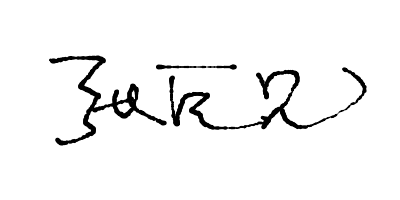
\includegraphics[height=1.5\baselineskip]{signature.png}
\end{flushright}
\clearpage

% Abstract
\begin{abstract}
The objective of this report is to present formalization of some basic theorems from transcendental number theory with {\tt \small Lean} and {\tt \small mathlib} in the hope that it will motivate and inspire other mathematicians, by igniting their curiosity about interactive theorem proving. The following theorems are formalized:
\begin{enumerate}
  \item the set of algebraic numbers is countable, hence transcendental number exists:

\begin{minted}[mathescape,linenos,numbersep=5pt,frame=single,framesep=2mm,fontsize=\footnotesize]{Lean}
theorem algebraic_set_countable : set.countable algebraic_set
theorem transcendental_number_exists : 
  ∃ x : ℝ, transcendental x
\end{minted}

  \item all Liouville numbers are transcendental:
\begin{minted}[mathescape,linenos,numbersep=5pt,frame=single,framesep=2mm,fontsize=\footnotesize]{Lean}
theorem liouville_numbers_transcendental : 
  ∀ x : ℝ, liouville_number x -> transcendental x
\end{minted}

  \item $\alpha := \sum_{i=0}^\infty\frac1{10^{i!}}$ is a Liouville number hence $\alpha$ is transcendental.

\begin{minted}[mathescape,linenos,numbersep=5pt,frame=single,framesep=2mm,fontsize=\footnotesize]{Lean}
theorem liouville_α : liouville_number α
theorem transcendental_α : transcendental α := 
  liouville_numbers_transcendental α liouville_α
\end{minted}

  \item $e$ is transcendental:
\begin{minted}[mathescape,linenos,numbersep=5pt,frame=single,framesep=2mm,fontsize=\footnotesize]{Lean}
theorem e_transcendental : transcendental e
\end{minted}
\end{enumerate}
\end{abstract}

% \section* {Disclaimer}
% The plan is to a self-contained report so that after chapter \ref{intro:lean} any reader even without prior exposure to interactive theorem proving will be able to understand \ref{fmlsn} where the details of formalizations and proofs reside. This should be relatively straightforward since the author is a {\tt \small Lean}-dilettantes at best with only a partial picture of the full language. For the same reason, much of the code is perhaps not idiomatic or even plainly bad, thus it is not advisable to use this as a tutorial.

\tableofcontents

\chapter{Overview}
\section{Interactive theorem proving}
Around 1920s, the German mathematician David Hilbert put forward a programme to seek:
\begin{enumerate}
  \item an axiomatic foundation of mathematics;
  \item a proof of consistency of the said foundation;
  \item Entscheidungsproblem: an algorithm to determine if any proposition is universally valid given a set of axioms.
\end{enumerate}
The first two aims were later proved to be impossible by Gödel and his celebrated incompleteness theorems. Via the completeness of first order logic, the Entscheidungsproblem can also be interpreted as an algorithm for producing proofs using deduction rules. Even without a panacea approach for mathematics, a computer still bears advantages against a carbon-based mathematician. Perhaps the most manifested advantage is the accuracy of a computer with which it execute its command and to recall its memories. Thus came the idea of {\bf interactive theorem proving} --- instead of hoping a computer algorithm can spit out some unfathomable proofs, assuming computers are given the ability to check the correctness of proofs, so human-comprehensible proofs can be verified by machines and thus guaranteed to be free of errors. With a collective effort, all theorems verified this way can be collected in an error-free library such that all mathematicians can utilise to prove further theorems, which can then be added to the collection, ad infinitum \cite{boyer1994qed}. Curry-Howard isomorphism provided the crucial relationship between mathematical proofs and computer programmes, more specifically relationship between propositions and types, to make such project feasible \cite{kennedy2011set}. The idea will be explained in section \ref{intro:lean} along with {\tt \small Lean}. 

The proof of ``Kepler's conjecture\footnote{the most efficient way to pack spheres should be hexagonally}'' illustrates and exemplifies the utility of interactive theorem proving. As early as 1998, Thomas Hales had claimed a proof \cite{hales1998kepler,harrison2014history}, however the proof is controversial in the sense that other mathematician even after great effort could not guarantee its correctness. A collaborative project using {\tt \small Isabelle}\footnote{a theorem prover relies extensively on dependent type theory and Curry-Howard correspondence.} and {\tt \small HOL Light}\footnote{ibid.} verified the proof around 2014, hence settled the controversy in 2017 \cite{hales2017formal}. There is also Georges Gonthier with his teams using {\tt \small Coq}\footnote{ibid.} who formalised the four colour theorem and Feit-Thompson theorem where the latter is a step closer to the classification of simple groups \cite{gonthier2008formal, gonthier2013machine}. Additionally, using {\tt \small Lean}\footnote{ibid.}, \Citeauthor{buzzard2020formalising} were able to formalise the modern notion of perfectoid spaces \cite{buzzard2020formalising}.

\section{History of transcendental numbers}

``Transcendence'' as a mathematical jargon first appeared in a Leibniz's 1682 paper where he proved that sine is a transcendental function in the sense that for any natural number $n$ there does not exist polynomials $p_0,\cdots,p_n$ such that
$$p_0(x)+p_1(x)\sin(x)+p_2(x)\sin(x)^2+\cdots+p_n(x)\sin(x)^n=0$$
holds for all $x\in\mathbb R$ \cite{bourbaki1998elements}. The Swiss mathematician Johann Heinrich Lambert in his 1768 paper proved the irrationality of $e$ and $\pi$ and he also conjectured their transcendence \cite{lambert2004memoire}. It is not until 1844 that Joseph Liouville proved the existence of any transcendental number and until 1851 an explicit example of transcendental number was actually given by its decimal expansion:\cite{10.2307/1988833}
$$\sum_{i=1}^\infty\frac1{10^{i!}}=0.11000100000\cdots.$$
However, this construction is still artificial in nature. The first example of a real number proven to be transcendental that is not constructed for the purpose of being transcendental was $e$. Charles Hermite proved the transcendence of $e$ in 1873 with a method applicable (with help of symmetric polynomial) to $\pi$ in 1882 and later to be generalised to Lindemann-Weierstrass theorem in 1885 stating that if $\alpha_1,\cdots, \alpha_n$ are distinct algebraic numbers then $e^{\alpha_1},\cdots,e^{\alpha_n}$ are linearly independent over the algebraic numbers \cite{baker1990transcendental}. The transcendence of $\pi$ was particularly celebrated because it immediately implied the impossibility of the ancient greek challenge of squaring the circle, i.e. it is not possible to construct a square, using compass and ruler only, with equal area to a circle. This question is plainly equivalent to construct $\sqrt\pi$, which is not possible for otherwise $\pi$ is algebraic. Georg Cantor in 1874 proved that algebraic numbers are countable hence not only do transcendental numbers exist, they exist in a ubiquitous manner -- there is a bijection from the set of all transcendental numbers to $\mathbb R$ \cite{cantor1932uber,cantor1878beitrag}.

In 1900, Hilbert proposed twenty-three questions, the 7th of which is regarding transcendental numbers: Is $a^b$ transcendental, for any algebraic number $a$ that is not $0$ or $1$ and any irrational algebraic number $b$? The answer is yes provided by Gelfond-Schneider theorem in 1934 \cite{gelfond1934septieme}. This led to some immediate consequences such that
\begin{enumerate}
  \item $2^{\sqrt2}$ and its square root ${\sqrt2}^{\sqrt2}$ are transcendental;
  \item $e^{\pi}$ is transcendental for $e^{\pi}=\left(e^{i\pi}\right)^{-i}=\left(-1\right)^{-i}$;
  \item $i^i=e^{-\frac\pi2}$ is transcendental etc.
\end{enumerate}
In contrast, none of $\pi\pm e$, $\pi e$,$\frac\pi e$, $\pi^\pi$, $\pi^e$, etc were proven to be transcendental. It was also conjectured by Stephen Schanuel that given any $n$ $\mathbb Q-$linearly independent $z_1,\cdots, z_n\in\mathbb C$, then $\mathrm{trdeg}\left(\mathbb Q(z_1,\cdots, zn, e^{z_1},\cdots, e^{z_n})/\mathbb Q\right)$ is at least $n$ \cite{lang1966introduction}. If this was proven, the algebraic independence of $e$ and $\pi$ would follow immediately by setting $z_1=1$ and $z_2=\pi i$ with Euler's identity.

\chapter{Brief introduction to {\tt Lean}}\label{intro:lean}

{\tt \small Lean} was developed by Leonardo de Moura at Microsoft Research Redmond in 2013 using dependent type theory and calculus of inductive constraint \cite{avigad2015theorem}. In this chapter, basic ideas of Curry-Howard isomorphism will be demonstrated by some basic examples of mathematical theorem expressed in {\tt \small Lean} using dependent type theory.

\section{Simple type theory}
Unlike set theory where everything from natural numbers to modular forms is essentially a set, type theory associate every expression with a {\tt \small type}. In set theory, an element can belong to different sets, for example $0$ is simultaneously in $\mathbb N\subseteq\mathbb Q\subseteq\mathbb R\subseteq\mathbb C$. However an expression can only have one type. $0$ without any context will have type $\mathbb N$ and, to specify the zero with type $\mathbb R$ we write $(0:\mathbb R)$. If $a$ has type $\alpha$, we write $a:\alpha$. By a universe of types we mean a collection of types. Types can be combined to form new types in the following way:
\begin{itemize}
  \item let $\alpha$ and $\beta$ be types then $\alpha\to\beta$ is the type of functions from $\alpha$ to $\beta$: the element of type $\alpha\to\beta$ is a function that for any element of $\alpha$ gives an element of $\beta$. For mathematicians this loosely means that for any two classes $\alpha$ and $\beta$, there is a new class $\hom(\alpha,\beta)$. Sometimes we are not bothered to give a function a name, we can use the $\lambda$ notation: the expression $(\lambda x:\alpha, \text{expression})$ has type $\alpha\to\dots$ depending on the content of expression. For example $(\lambda x:\mathbb N, x+1):\mathbb{N}\to\mathbb{N}$ is the function from natural numbers to natural numbers that add $1$ to any input.
  \item let $\alpha$ and $\beta$ be types then $\alpha\times\beta$ is the cartesian product of $\alpha$ and $\beta$: the element of type $\alpha\times\beta$ is an ordered tuple $(a,b)$ where $a:\alpha$ and $b:\beta$.
  \item Let $\alpha$ be a type in universe $\mathcal U$ and $\beta:\alpha\to\mathcal U$ be a family of type that for any $a:\alpha$, $\beta(a)$ is a type in $\mathcal U$. Then we can form the $\Pi$-type $$\prod_{a:\alpha}\beta(a)$$ whose element is of the form $f:\prod_{a:\alpha}\beta(a)$ such that for any $x:\alpha$, $f(x):\beta(x)$. Note that function type is actually an example of $\Pi$-type where $\beta$ is a constant family of types. For this reason, we also call $\Pi$-types dependent functions. For example if $\mathrm{Vec}(\mathbb{R},n)$ is the type of $\mathbb R^n$, then 
    $$n\mapsto\underbrace{(1,\cdots,1)}_{n\text{ times}}:\prod_{m:\mathbb N} \mathrm{Vec}(\mathbb R, m)$$
  \item We also have dependent cartesian product or $\Sigma$-type: Let $\alpha$ be a type in universe $\mathcal U$ and $\beta:\alpha\to\mathcal U$ be a family of types in $\mathcal U$, then the $\Sigma$-type $$\sum_{a:\alpha}\beta(a)$$ whose element is of the form $(x,y):\sum_{a:\alpha}\beta(a)$ such that $x:\alpha$ and $y:\beta(x)$. Similarly $$\left(n,\underbrace{(1,\cdots,1)}_{n\text{ times}}\right):\sum_{m:\mathbb N} \mathrm{Vec}(\mathbb R, m)$$
\end{itemize}

\subsection{Proposition as type}
In type theory, a proposition $p$ can be regarded as a type whose elements is a proof of $p$.

\begin{example}
$1+1=2$ is a proposition. {\tt \small rfl} is an element of type $1+1=2$ where {\tt \small rfl} is the assertion that every term equals to itself.
\end{example}

\begin{example}
For two propositions $p$ and $q$, the implication $p\implies q$ then can be interpreted as function $p\to q$. To say $\mathrm{imp}: p\to q$ is to say for any $\mathrm{hp}:p$ we have $\mathrm{imp}( \mathrm{hp}): q$, or equivalently given any $\mathrm{hp}$, a {\it proof} of proposition $p$, $\mathrm{imp}(\mathrm{hp})$ is a proof of proposition $q$. 
\end{example}

\begin{example}
If $p:\alpha\to\mathrm{proposition}$, the proposition
$\forall x : \alpha, p(x)$ can be interpreted as a $\Pi$-type $\prod_{x:\alpha} p(x)$. To prove $\forall x: \alpha, p(x)$, we need to find an element of type $\prod_{x:\alpha} p(x)$; equivalently for any $x:\alpha$, we need to find an element of type $p(x)$; equivalently for any $x:\alpha$, we need to find a proof of $p (x)$.

Similarly, $\exists x:\alpha, p(x)$ can be interpreted as a $\Sigma$-type $\sum_{x:\alpha} p(x)$. To prove $\exists x:\alpha, p(x)$ is to find an element $x$ of type $\alpha$ and prove $p(x)$, equivalent to find an element $x:\alpha$ and an element of type $p(x)$ and this is precisely $(x, p(x)):\sum_{a:\alpha} p(a)$.
\end{example}

Theorems are true propositions. Using the interpretation above, theorems are inhabited types and to prove a theorem is to find an element of the required type.

\section{{\tt Lean} and {\tt mathlib}}
{\tt \small mathlib} is the collection of mathematical definitions, theorems, lemmas built on {\tt \small Lean}. {\tt \small mathlib} includes topics in algebra, topology, manifolds and combinatorics etc. The following section will briefly explain how to use {\tt \small Lean} with {\tt \small mathlib}.


In {\tt \small Lean}, new definition can be introduced with the following syntax:
\begin{minted}[mathescape,linenos,numbersep=5pt,frame=single,framesep=2mm,breaklines,escapeinside=||]{Lean}
def name (arg|$_1$|:type|$_1$|) ... (arg|$_n$|:type|$_n$|) : return_type := contents

def name' {arg|$_1$|:type|$_1$|} ... (arg|$_n$|:type|$_n$|) : return_type := contents
\end{minted}
{\tt \small return\_type} is optional when it can be inferred from {\tt \small contents}. If an argument is enclosed by curly brackets instead of round brackets, then when the definition is invoked the said argument is implicit, i.e. {\tt \small name' a$_2$ ... a$_n$} where {\tt \small a$_i$:type$_i$}. To explicitly mention the said argument, one needs to use {\tt \small @name' a$_1$ ... a$_n$} where {\tt \small a$_i$:type$_i$}. One can use ``if then else'' to introduce a function whose value depends on the value of the arguments:
\begin{minted}[mathescape,linenos,numbersep=5pt,frame=single,framesep=2mm,breaklines,escapeinside=||]{Lean}
def name args : return_type :=
  if (h args)
  then contents|$_1$|
  else contents|$_2$|

def name args : return_type := 
  ite (h args) contents|$_1$| contents|$_2$|
\end{minted}

New notations are introduced with the following syntax:
\begin{minted}[mathescape,linenos,numbersep=5pt,frame=single,framesep=2mm,breaklines,escapeinside=§§]{Lean}
notation _`lhs`_ := _rhs_
\end{minted}
so that {\tt \small Lean} will treat every occurrence of {\tt \small \_`lhs`\_} as {\tt \small \_rhs\_} verbatim. For example \mintinline{Lean}{notation ℤ`[X]` := polynomial ℤ} will replace the {\tt \small Lean} type {\tt \small polynomial ℤ} with a more familiar notation of $\mathbb{Z}[X]$.

For any type of $\alpha$, we can introduce a subtype of $\alpha$ by:
\begin{minted}[mathescape,linenos,numbersep=5pt,frame=single,framesep=2mm,breaklines,escapeinside=§§]{Lean}
def α' := {x : α // property_satisfied_by_x}
\end{minted}
An element of type $\alpha'$ is of the form $\langle x, hx\rangle$ where $x:\alpha$ and $hx$ is a proof that $x$ satisfies the given property.

Theorems or lemmas are introduced with the following syntax:
\begin{minted}[mathescape,linenos,numbersep=5pt,frame=single,framesep=2mm,breaklines,escapeinside=||]{Lean}
theorem name (arg|$_1$|:type|$_1$|) ... (arg|$_n$|:type|$_n$|) : content :=
begin
  -- proof of the theorem
end
\end{minted}

To write a proof understandable to {\tt \small Lean}, one need to use {\it tactic mode}. In {\tt \small Lean}, one can use
\begin{itemize}
  \item proof by induction: if the goal is a proposition about natural number $n$, {\tt \small induction n with n IH} is to prove the proposition by induction. This command will change the current goal to two goals. The first is to prove the proposition for $n=0$ and the second to prove the proposition $n+1$ with the additional inductive hypothesis {\tt \small IH};

\begin{minted}[mathescape,linenos,numbersep=5pt,frame=single,framesep=2mm,breaklines,escapeinside=||]{Lean}
theorem awesome_theorem_about_natural_number (n : ℕ) : proposition|$_\mathtt{n}$| :=
begin
  induction n with n IH,

  a_proof_of_proposition|$_\mathtt{0}$|

  -- (IH : proposition$_\mathtt{n}$) is now in context
  a_proof_of_proposition|$_\mathtt{n+1}$|
end
\end{minted}

  \item proof by contradiction: if the goal is to prove proposition $H$, {\tt \small by\_contra absurdum} will add {\tt \small absurdum : $\neg H$} into the current context and turn the goal into proving {\tt \small false};

\begin{minted}[mathescape,linenos,numbersep=5pt,frame=single,framesep=2mm,breaklines,escapeinside=||]{Lean}
theorem awesome_theorem : awesome_proposition :=
begin
by_contra absurdum,

-- Now (absurdum : $\neg$ awesome_proposition) is in context and the goal is to prove falsehood.
a_proof_of_falsehood
end
\end{minted}
  \item proof in a forward manner i.e. introduce new theorem into the current context or convert known theorem in the current context to approach the goal:
  \begin{itemize}
    \item {\tt \small have H := content} will introduce a new proposition whose proof is given by {\tt \small content}.
    
    {\tt \small have H : some\_proposition} will add one more goal of proving the proposition then introduce the proved proposition to the current context.

    \item If {\tt \small H} is in context then {\tt \small replace H := content} will change {\tt \small H} to (a proof of) the proposition that {\tt \small content} is proving.
    
    {\tt \small replace H : some\_proposition} will add one more goal of proving {\tt \small some\_proposition} and then replace {\tt \small H} to the proposition proven.
    \item If {\tt \small H} is in context, {\tt \small simp at H} will simplify {\tt \small H} to using small lemmas\footnote{to be more precise, lemma with {\tt \scriptsize @[simp]} tag, i.e. lemmas declared in the following syntax {\tt \scriptsize @[simp] lemma lemma\_name args : Prop}. These lemma are usually trivial in nature such as {\tt \scriptsize nat.add\_zero} which asserts that $\forall n:\mathbb N, n + 0 = n$.}.
    {\tt \small simp only [h1,\dots,hn]} is to simplify only using {\tt \small h1 }\dots{\tt \small{ hn}}.
    \item {\tt \small rw} is for term rewriting. If we have {\tt \small h : lhs = rhs} or {\tt \small h : lhs<->rhs} and another {\tt \small H} in context, then {\tt \small rw h at H} will replace every occurrence of {\tt \small lhs} with {\tt \small rhs} in {\tt \small H} and {\tt \small rw <-h} will replace every occurrence of {\tt \small rhs} with {\tt \small lhs} in {\tt \small H}.
  
    {\tt \small rw [h1, h2,..., hn] at H} is the same as {\tt \small rw h1 at H, rw h2 at H,..., rw hn at H}.
    
    \item The fact that {\tt \small rw} and {\tt \small simp} change all term occurrences sometimes creates an inconvenience. If {\tt \small H} is in context, {\tt \small conv\_lhs at H \{tactics\}} will confine the scope of {\tt \small tactics} only to the left hand side of H; similarly {\tt \small conv\_rhs at H \{tactics\}} will confine the scope to the right hand side of H.

    \item {\tt \small generalise H : lhs = var\_name} will set {\tt \small var\_name} to {\tt \small lhs} and add (proof of) the proposition {\tt \small H : lhs = var\_name} to the current context.
    \item If {\tt \small H : ∃ x : type, property\_about\_x} is in the current context, {\tt \small choose x hx using H} will introduce {\tt \small x:type} with the assumption {\tt \small property\_about\_x} to the current context. 
    \item If {\tt \small H : $p\land q$} is in the current context, then {\tt \small H.1} is (a proof of) $p$ and {\tt \small H.2} is (a proof of) $q$.
    \item If {\tt \small H : ite h1 h2 h3} is in the current context, then {\tt \small split\_ifs at H} will turn the current goal into two goals, the first one is to prove the original goal with the additional assumption {\tt \small h1} and {\tt \small h2}; the second one is to prove the original with goal with the additional assumption {\tt \small $\neg$h1} and {\tt \small h3}.
  \end{itemize}

  \item proof in a backward manner i.e. convert or replace the goal so that it is closer to what is known in context:
  \begin{itemize}
    \item {\tt \small unfold definition} is to unfold a definition to what is explicitly defined when the definition is introduced.
    \item {\tt \small simp}, {\tt \small rw}, {\tt \small conv\_lhs \{tactics\}} and {\tt \small conv\_rhs \{tactics\}} is the same as above except now they change at goal.
    \item Given (a proof of) proposition {\tt \small H: h1 -> h2}, then {\tt \small apply H} will change the goal of proving {\tt \small h2} to prove {\tt \small h1}.
    \item {\tt \small suffices H : some\_proposition} ask for a proof of the current goal with additional {\tt \small H}, then ask for a proof of {\tt \small H}.
    \item {\tt \small norm\_cast} converts the type of numbers. For example the current goal is $(x:\mathbb R)<(y:\mathbb R)$ where $x$ and $y$ are of type $\mathbb N$, then after {\tt \small norm\_cast} the goal will become $x<y$. This should be simpler because $\mathbb R$ in {\tt \small Lean} is defined as equivalent classes of Cauchy sequence of $\mathbb Q$ while natural number is much easier to work with.
    
    {\tt \small norm\_num} is equivalent to {\tt \small norm\_cast, simp}.

    \item {\tt \small ext} will convert the current goal with axioms of extensionality. For example if the goal is to prove equality of polynomial then after {\tt \small ext} the goal would become to prove that every coefficient is equal; or if the goal is to prove equality of sets of type $\alpha$ $A=B$, then after {\tt \small ext}, an arbitrary element {\tt \small x} of type $\alpha$ will be introduced into context then the goal will become to prove $x\in A\iff x\in B$. {\tt \small ext var\_name} will force {\tt \small Lean} to introduce a new variable under the identifier {\tt \small var\_name}.
    \item If the goal is to prove {\tt \small ite h1 h2 h3} (or {\tt \small ite h1 h2 h3 = rhs}), then {\tt \small split\_ifs at H} will turn the current goal into two goals, the first one is to prove {\tt \small h2} ({\tt \small h3 = rhs} resp.) with the additional assumption {\tt \small h1}; the second one is to prove {\tt \small h3} ({\tt \small h3 = rhs} resp.) with the additional assumption {\tt \small $\neg$h1}
  \end{itemize}

  \item when the goal is easily provable, one can use the following to finish a goal:
  \begin{itemize}
    \item {\tt \small refl} (for reflexive) is used to prove propositions of the form {\tt \small lhs = rhs} when {\tt \small lhs} is {\bf definitionally} equal to {\tt \small rhs}. Definitional equality is more general than two string being literally identical but is less general than being (canonically) isomorphic. For example
    $$
  \sum_{i=0}^\infty \frac{1}{2^i}=\sum_{j=0}^\infty \frac{1}{2^j}
    $$
    is a definitional equality but
    $$
  \mathbb R^n = \mathrm{Func}\left(\{0,\cdots, n-1\},\mathbb R\right)
    $$ is not a definitional equality (strictly speaking perhaps not an equality at all).
    \item {\tt \small exact H} will prove the current goal if the goal is definitionally equal to {\tt \small H}. 
  
    \item {\tt \small ring} will try to prove the current goal using associativity and commutativity of addition and multiplication.
    \item {\tt \small linarith} is used when proving inequality from context. {\tt \small linarith} is semi-automated, so it can work with inequalities with symbols or variables but only to a degree. If {\tt \small linarith} fails, one has to either provide {\tt \small linarith} with more propositions or use other tactics to change the goal into something more manageable the use {\tt \small linarith}.
  
    {\tt \small linarith [h1, ..., hn]} is equivalent to use {\tt \small linarith} with additional (proofs of) propositions {\tt \small h1} \dots {\tt \small { hn}}.
    \item {\tt \small tidy} is to ask {\tt \small Lean} to try different tactics and finishes the goal if it possible.
  \end{itemize}

  \item If there is multiple goals, one can use {\tt \small \{ \}} to focus on the first one.
  \item If the entirety of proof is one line, one can replace {\tt \small begin contents end} with {\tt \small by contents}.
\end{itemize}


A proposition if not atomic is either a conjunction, a disjunction, an implication, an equivalence, a negation or a proposition with universal quantifier or existential quantifier.

\subsection*{prove a conjunction}\label{lean:conj}
If the goal is to prove a conjunction of the form $h_1 \land h_2$, {\tt \small split} is used. It will change the current goal to two goals of proving $h_1$ and $h_2$ respectively. Then the general pattern is

\begin{minted}[mathescape,linenos,numbersep=5pt,frame=single,framesep=2mm,breaklines,escapeinside=||]{Lean}
theorem how_to_prove_conjunction (|$h_1$| : Prop) (|$h_2$| : Prop) : |$h_1\land h_2$| :=
begin
split,

proof_of_|$h_1$|

proof_of_|$h_2$|
end
\end{minted}


\subsection{prove a disjunction}\label{lean:disjun}
If the goal is to prove a disjunction of the form $h_1 \lor h_2$, one can use {\tt \small left} to change the goal to prove $h_1$ or {\tt \small right} to change the goal to prove $h_2$. Let us assume $h_1$ is a true proposition :

\begin{minted}[mathescape,linenos,numbersep=5pt,frame=single,framesep=2mm,breaklines,escapeinside=||]{Lean}
theorem how_to_prove_disjunction (|$h_1$| : Prop) (|$h_2$| : Prop) : |$h_1\lor h_2$| :=
begin
left,
  
proof_of_|$h_1$|
end
\end{minted}


\subsection{prove an implication}\label{lean:imp}
If the goal is to prove an implication of the form $p \implies q$, one can use {\tt \small intro h$p$} to add {\tt \small h$p$:$p$} a proof of $p$ into the context and convert the goal to proving $q$.

\begin{minted}[mathescape,linenos,numbersep=5pt,frame=single,framesep=2mm,breaklines,escapeinside=||]{Lean}
theorem how_to_prove_implication (|$p$| : Prop) (|$q$| : Prop) : |$p$| -> |$q$| :=
begin
intro h|$p$|,
  
proof_of_|$q$|
end
\end{minted}

If the goal is of the form $p_1\to p_2\to\dots p_n$, one can use {\tt \small intros h$p_1$ \dots h$p_n$} as an abbreviation of {\tt \small intro h$p_1$, intro h$p_2$,\dots, intro h$p_n$}.


\subsection{prove an equivalence}\label{lean:eqv}
An equivalence of the form $p \iff q$ is by definition $p\implies q \land q\implies p$. Thus {\tt \small split} will change the goal to two goals, one to prove $p\implies q$, the other to prove $q \implies p$. Then use section \ref{lean:imp}.

\subsection{prove a negation}
A negation of the form $\neg p$ is by definition $p \implies \bot$. Thus {\tt \small intro h$p$} will add {\tt \small h$p$:$p$} to the current context and convert the goal to proving a falsehood.

\begin{minted}[mathescape,linenos,numbersep=5pt,frame=single,framesep=2mm,breaklines,escapeinside=||]{Lean}
theorem how_to_prove_negation (|$p$| : Prop) : |$\neg p$| :=
begin
intro h|$p$|,

proof_of_falsehood
end
\end{minted}

\subsection{prove a proposition with $\forall$}\label{lean:forall}
A proposition of the form $\forall a : \alpha, p(a)$ where $\alpha$ is a type and $p : \alpha\to$ {\tt \small Prop} can be proved also using {\tt \small intro $x_0$}. This will add an arbitrary $x_0:\alpha$ to the current context and change the goal to proving $p(x_0)$.

\begin{minted}[mathescape,linenos,numbersep=5pt,frame=single,framesep=2mm,breaklines,escapeinside=||]{Lean}
theorem how_to_proposition_with_universal_quantifier {|$\alpha$| : Type} (|$p$| : |$\alpha$| -> Prop) : ∀ a : α, p a :=
begin
intro |$x_0$|,

a_proof_of_|$p(x_0)$|
end
\end{minted}

If the goal is the form $\forall a_1:\alpha_1,\forall a_2:\alpha_2,\dots,\forall a_n:\alpha_n, p\ a_1\ a_2\ \dots\ a_n$ can be proved using {\tt \small intros $a_1$ $a_2$ \dots\  $a_n$} as an abbreviation of {\tt \small intro $a_1$, intro $a_2$,\dots, intro $a_n$}.

\subsection{prove a proposition with $\exists$}\label{lean:exists}
A proposition of the form $\exists a:\alpha, p(a)$ where $\alpha$ is a type and $p : \alpha\to$ {\tt \small Prop}  can be proved by {\tt \small use $x_0$}. This will convert the goal to proving $p(x_0)$.

\begin{minted}[mathescape,linenos,numbersep=5pt,frame=single,framesep=2mm,breaklines,escapeinside=||]{Lean}
theorem how_to_proposition_with_universal_quantifier {|$\alpha$| : Type} (|$p$| : |$\alpha$| -> Prop) : ∃ a : α, p a :=
begin
a_construction_of_|$x_0$|

use |$x_0$|,
  
a_proof_of_|$p(x_0)$|
end
\end{minted}

\section{An example}
To illustrate the above syntax and patterns, an example is presented here of defining mean value of two real numbers and proving some basic properties thereof.

\begin{minted}[mathescape,linenos,numbersep=5pt,frame=single,framesep=2mm,breaklines,escapeinside=||]{Lean}
import data.real.basic |\label{import:real}|
import tactic |\label{import:tactic}|
  
noncomputable theory |\label{noncomputable}|
open_locale classical |\label{proof_by_contradiction}|  

def mean (x y : ℝ) : ℝ := (x + y) / 2 |\label{example:def}|
  
theorem min_le_mean : ∀ x y : ℝ, min x y ≤ (mean x y) := |\label{example:thm_begin}|
begin
intros x y,
have ineq1 : min x y ≤ x := min_le_left x y,
have ineq2 : min x y ≤ y := min_le_right x y,
    
unfold mean, rw le_div_iff, rw mul_two, 
apply add_le_add, 
exact ineq1, exact ineq2, 
  
linarith,
end
  
theorem mean_le_max : ∀ x y : ℝ, (mean x y) ≤ max x y :=
begin
intros x y,
have ineq1 : x ≤ max x y := le_max_left x y,
have ineq2 : y ≤ max x y := le_max_right x y,
  
unfold mean, rw div_le_iff, rw mul_two,
apply add_le_add,
exact ineq1, exact ineq2,
  
linarith,
end |\label{example:thm_end}|
  
theorem a_number_in_between : 
  ∀ x y : ℝ, x ≤ y -> ∃ z : ℝ, x ≤ z ∧ z ≤ y :=
begin
intros x y hxy,
have ineq1 := min_le_mean x y,
have ineq2 := mean_le_max x y,
have min_eq_x := min_eq_left hxy,
have max_eq_y := max_eq_right hxy,
use mean x y,
split,
  
{ conv_lhs {rw <-min_eq_x}, exact ineq1, },
{ conv_rhs {rw <-max_eq_y}, exact ineq2, },
end

\end{minted}

Line \ref{import:real} makes basic properties of real available to use and line \ref{import:tactic} makes all the tactics we discussed amongst other more advanced tactics available to use. We add line \ref{noncomputable} so that {\tt \small lean} would ignore the issue of computability and line \ref{proof_by_contradiction} so that we can use proof by contradiction\footnote{{\tt \small Lean} by default use constructivism where $\neg\neg p\implies p$ is not an axiom of deduction. Thus the law of excluded middle is not by default a tautology.}. 

We define the mean value of two real numbers on line \ref{example:def}. Then {\tt \small mean}\footnote{{\tt \small mean} is not a function $\mathbb R^2\to\mathbb R$ but a function $\mathbb R\to\mathrm{Func}(\mathbb R,\mathbb R)$. This is called currying.} has the type $\mathbb R\to \mathbb R\to \mathbb R$, {\tt \small mean 1} has the type $\mathbb R\to \mathbb R$ and {\tt \small mean 1 2} has the type $\mathbb R$. 

We can introduce and prove theorems about {\tt \small mean} stating that the mean value of two numbers is greater than or equal to the minimum of the two numbers but less than the maximum. This is from line \ref{example:thm_begin} to line \ref{example:thm_end} where
\begin{itemize}
  \item {\tt \small min\_le\_left} is a proof of the proposition $\forall (x\ y : \alpha), \min(x, y) \le x$ where $\alpha$ is an implicit argument with a linear order. In this case, {\tt \small Lean} infers from context that $\alpha$ is $\mathbb R$. Thus {\tt \small min\_le\_left x y} is a proof of {\tt \small min x y ≤ x}.
  \item {\tt \small min\_le\_right} is a proof of the proposition $\forall (x\ y : \alpha), \min(x, y) \le y$ In this case, {\tt \small min\_le\_right x y} is a proof of {\tt \small min x y ≤ y}.
  \item Similarly, {\tt \small le\_max\_left} is a proof of the proposition $\forall (x\ y : \alpha), x \le \max(x, y)$ where $\alpha$ is an implicit argument with a linear order. In this case, {\tt \small le\_max\_left} is a proof of {\tt \small x ≤ max x y}.
  \item Similarly, {\tt \small le\_max\_right} is a proof of the proposition $\forall (x\ y : \alpha), y \le \max(x, y)$ where $\alpha$ is an implicit argument with a linear order. In this case, {\tt \small le\_max\_right} is a proof of {\tt \small y ≤ max x y}.
  \item {\tt \small le\_div\_iff} is a proof that $0 < c \to (a \le \frac{b}{c} \iff a\times c \le b)$ where $a,b,c$ are elements of a type with a linear ordered field structure. So by {\tt \small rw le\_div\_iff}, the goal would change from {\tt \small min x y ≤ (x + y) / 2} to {\tt \small min x y * 2 ≤ x + y}. Since {\tt \small le\_div\_iff} requires the assumption that $0<c$, a new goal to prove that {\tt \small 0 < 2} is created after the original goal. This goal is proved by the final {\tt \small linarith}.
  \item {\tt \small div\_le\_iff} is proof that $0 < b \implies (\frac a b \le c \iff a \le c \times b)$ where $a,b,c$ are elements of a type with a linear ordered field structure. So by {\tt \small rw div\_le\_iff} the goal would change from {\tt \small (x + y) / 2 ≤ max x y} to {\tt \small x + y ≤ max x y * 2}. Since {\tt \small div\_le\_iff} requires the assumption that $0 < b$, a new goal to prove $0 < 2$ is created after the original goal. This goal is proved by the final {\tt \small linarith}.
  \item {\tt \small mul\_two} proves the lemma that $\forall n:\alpha, n\times 2 = n+n$ where $\alpha$ is a semiring. Thus {\tt \small rw mul\_two} would change the goal of proving {\tt \small min x y * 2 ≤ x + y} ({\tt \small x + y ≤ max x y * 2} resp.) to {\tt \small min x y + min x y ≤ x + y} ({\tt \small x + y ≤ max x y + max x y} resp.).
  \item {\tt \small add\_le\_add} proves the lemma that $a \le b \to c \le d \to a + c \le b + d$ where $a$, $b$, $c$ and $d$ are elements of an ordered additive commutative monoid. Since the goal now is to prove {\tt \small min x y + min x y ≤ x + y}, by {\tt \small apply add\_le\_add}, goal will be replaced by two goals of proving {\tt \small min x y ≤ x} and {\tt \small min x y ≤ y}. These are {\it exactly} {\tt \small ineq1} and {\tt \small ineq2}.
\end{itemize}

\chapter{Formalisation using {\tt Lean}}\label{fmlsn}

\section*{Logistics of the formalisation}
\addcontentsline{toc}{section}{Logistics of the formalisation}
There are five main files in this project where 
\begin{enumerate}
\item {\tt \small small\_things.lean} formalised results about the trivial embedding of $\mathbb Z[X]\subset \mathbb R[X]$ and manipulation of inequality in real numbers common to all three parts;
\item {\tt \small algebraic\_over\_Z.lean} formalised countability of algebraic numbers with help of Schröder-Berstein theorem.
\item {\tt \small liouville.lean} formalised Liouville's theorem and a construction of a Liouville's number;
\item {\tt \small e\_trans\_helpers2.lean} formalised some results about differentiation and integration. Especially the formalisations of 
$$
\frac{\mathrm d^n}{\mathrm d x^n}uv = \sum_{i=0}^n{n \choose i}\frac{\mathrm d^i u}{\mathrm d x^i}\frac{\mathrm d^{n-i} v}{\mathrm d x^{n-i}}
$$ where $u$ and $v$ are differentiable function from $\mathbb R$ to $\mathbb R$ and
$$
\int_0^t e^{t-x}f(x)\mathrm{d}x=e^t\sum_{i=0}^m f^{(i)}(0)-\sum_{i=0}^m f^{(i)}(t)
$$ where $f(X)\in\mathbb Z[X]$;
\item {\tt \small e\_transcendental.lean} formalised transcendence of $e$ by assuming the algebraicity of $e$ which resulted in two contradictory bounds using the results from {\tt \small e\_trans\_helpers2.lean}.
\end{enumerate}

\section{Countability argument}\label{fmlsn:count}
The main caveat in this part is the internal specification of {\tt \small mathlib}. 
A real number $x$ in {\tt \small Lean} is algebraic over $\mathbb Z$ if and only if there exists a nonzero polynomial $p(X)\in\mathbb Z[X]$ such that $p$ is in the kernel of the unqiue $\mathbb Z$-algebra homomorphism $\mathbb Z[X]\to\mathbb R$ given by $X\mapsto x$.
\begin{minted}[mathescape,linenos,numbersep=5pt,frame=single,framesep=2mm,breaklines,escapeinside=||]{Lean}
∃ (p : ℤ[X]), p ≠ 0 ∧ |$\Uparrow$|(polynomial.aeval ℤ ℝ x) p = 0
\end{minted}
Here the $\mathbb Z$-algebra homomorphism is {\tt \small polynomial.aeval ℤ ℝ x}. $\Uparrow$ is to convert the homomorphism to a function applicable to {\tt \small p}. The reason that a conversion is necessary is because an algebra homomorphism contains more information than a function, it is a structure containing the map and other fields containing (proofs of) the properties of algebra homomorphism.
However in polynomial library of {\tt \small mathlib}, the definition of root is as following :

\begin{minted}[mathescape,linenos,numbersep=5pt,frame=single,framesep=2mm,breaklines,escapeinside=||]{Lean}
def is_root (p : polynomial R) (a : R) : Prop := p.eval a = 0
\end{minted}

Thus the first part of this formalisation is to unify the two evaluation methods -- denote $\iota_x$ to be the unique $\mathbb Z$-algebra homomorphism $\iota_x : \mathbb Z[X]\to\mathbb R$ given by $X\to x$ then for all polynomial $p(X)\in\mathbb Z[X]$ and for all $x\in\mathbb R,\mathrm{eval}_p(x) = \iota_x p$:

\begin{code}
\begin{minted}[mathescape,linenos,numbersep=5pt,frame=single,framesep=2mm,breaklines,escapeinside=||]{Lean}
-- the trivial embedding $\mathbb{Z}[X]\subseteq\mathbb{R}[X]$
def poly_int_to_poly_real (p : ℤ[X]) : polynomial ℝ := polynomial.map ℤembℝ p
    
def poly_int_to_poly_real_wd (p : ℤ[X]) := 
  ∀ x : ℝ, polynomial.aeval ℤ ℝ x p = (poly_int_to_poly_real p).eval x
    
theorem poly_int_to_poly_real_well_defined |\label{codethm:countableUnify}|
  (x : ℝ) (p : ℤ[X]) : poly_int_to_poly_real_wd p :=
begin
  proof_omitted
end
\end{minted}
\caption{unifying two ways of evaluation}
\label{code:countableUnify}
\end{code}

For any $p\in\mathbb Z[X]$, we can define the set of roots to be $\{x \in\mathbb R | \mathrm{eval}_p(x) = 0\}$ or $\{x\in\mathbb R| \iota_x p=0\}$ where the former is builtin as {\tt \small $\uparrow$(poly\_int\_to\_poly\_real p).roots}\footnote{{\tt \small \_.roots} in fact has type {\tt \small finset ℝ}. The type {\tt \small finset} is a {\tt \small set} with a proof of finite cardinality. Here $\uparrow$ is used to convert a {\tt \small finset} to {\tt \small set} by discarding the proof of finite cardinality.} and the latter is defined as line \ref{code:rootsDef} in source code \ref{lst:rootsDef}. By line \ref{codethm:countableUnify} in source code \ref{code:countableUnify}, the two sets must be equal, hence they have finite cardinality:

\begin{code}
\begin{minted}[mathescape,linenos,numbersep=5pt,frame=single,framesep=2mm,breaklines, escapeinside=§§]{Lean}
def roots_real (p : ℤ[X]) : set ℝ := §\label{code:rootsDef}§
  {x | polynomial.aeval ℤ ℝ x p}

theorem roots_real_eq_roots (p : ℤ[X]) (hp : p ≠ 0) : 
  roots_real p = §$\uparrow$§(poly_int_to_poly_real p).roots :=
begin
  proof_omitted
end

theorem roots_finite (p : ℤ[X]) (hp : p ≠ 0) : 
  set.finite (roots_real p) :=
begin
  proof_omitted
end
\end{minted}
\caption{two ways of defining roots}
\label{lst:rootsDef}
\end{code}

We define the set of all algebraic numbers over $\mathbb Z$ to be
\begin{minted}[mathescape,linenos,numbersep=5pt,frame=single,framesep=2mm,breaklines, escapeinside=§§]{Lean}
def algebraic_set : set ℝ := {x | is_algebraic ℤ x}
\end{minted}
To investigate the countability of {\tt \small algebraic\_set}, we compare it with
\begin{equation}
  \bigcup_{n\in\mathbb N}\bigcup_{\substack{p\in\mathbb{Z}[X]\\ p\ne 0\\ \deg{p}<n+1}} \{x\in\mathbb{R}|\iota_xp=0\}.
  \label{countability:setEq}
\end{equation}


To this end, we introduce some types of interest:
\begin{minted}[mathescape,linenos,numbersep=5pt,frame=single,framesep=2mm,breaklines, escapeinside=§§]{Lean}
notation `int_n` n := fin n -> ℤ
notation `nat_n` n := fin n -> ℕ
notation `poly_n'` n := {p : ℤ[X] // p ≠ 0 ∧ p.nat_degree < n}
notation `int_n'` n := {f : fin n -> ℤ // f ≠ 0}
notation `int'` := {r : ℤ // r ≠ 0}
\end{minted}

where  $\langle m, hm\rangle$ is an element of {\tt \small fin n} if and only if $m$ is a natural number and $hm$ is a proof of $m < n$. Then {\tt \small fin n} is the type of only $n$ elements. Thus
\begin{itemize}
  \item {\tt \small int\_n n} is $\mathbb Z^n$;
  \item {\tt \small int\_n' n} is $\mathbb Z^n-\{(0,\dots,0)\}$;
  \item {\tt \small int'} is $\mathbb Z-\{0\}$;
  \item {\tt \small nat\_n n} is $\mathbb N^n$;
  \item {\tt \small poly\_n' n} is the type of non-zero integer polynomials with degree less than $n$.
\end{itemize}

Then $\mathbb Z\simeq \mathbb Z-\{0\}$ by the bijective function $s:\mathbb Z\to \mathbb Z-\{0\}$:
\begin{equation*}
n\mapsto\left\{
\begin{aligned}
& m & \text{if }m < 0\\
& m + 1 & \text{if }m \ge 0
\end{aligned}
\right.
\end{equation*}
\begin{code}
\begin{minted}[mathescape,linenos,numbersep=5pt,frame=single,framesep=2mm,breaklines, escapeinside=§§]{Lean}
def strange_fun : ℤ -> int' := 
  λ m, if h : m < 0 
       then ⟨m, by linarith⟩ 
       else ⟨m + 1, by linarith⟩

theorem strange_fun_inj : 
  function.injective strange_fun :=
begin
  proof_omitted
end

theorem strange_fun_sur : 
  function.surjective strange_fun :=
begin
  proof_omitted
end

theorem int_eqiv_int' : ℤ §$\simeq$§ int' :=
begin
  apply equiv.of_bijective strange_fun,
  split,
  exact strange_fun_inj,
  exact strange_fun_sur,
end
\end{minted}
\caption{$\mathbb Z\simeq \mathbb Z-\{0\}$}
\end{code}

Then we prove that for all non-zero $n:\mathbb N$, non-zero integer polynomials of degree less than $n$ bijectively correspond to $\mathbb Z^n-\{(0,\dots,0)\}$ via the function:
$p\mapsto \mathbf{z}$ where the $i$-th coordinate of $\mathbf{z}$ is the $i$-th coefficient of $p$.
\begin{code}
\begin{minted}[mathescape,linenos,numbersep=5pt,frame=single,framesep=2mm,breaklines, escapeinside=§§]{Lean}
def identify (n : nat) : (poly_n' n) -> (int_n' n) := 
  λ p, ⟨λ m, p.1.coeff m.1, a_proof_§$\mathbf{z}$§_is_not_zero⟩

theorem sur_identify_n (n : nat) (hn : n ≠ 0) : 
    function.surjective (identify n) :=
begin
  proof_omitted
end

theorem inj_identify_n (n : nat) (hn : n ≠ 0) : 
  function.injective (identify n) :=
begin
  proof_omitted
end

theorem poly_n'_equiv_int_n' (n : nat) : 
  (poly_n' n.succ) §$\simeq$§ (int_n' n.succ) :=
begin
  apply equiv.of_bijective (identify n.succ),
  split,
  exact inj_identify_n n.succ (nat.succ_ne_zero n),
  exact sur_identify_n n.succ (nat.succ_ne_zero n),
end
\end{minted}
$\dagger$: {\tt\small n.succ} means $n+1$.
\caption{non-zero integer polynomials with degree less than $n$ has the same cardinality as $\mathbb Z^n-\{(0,\dots,0)\}$}
\end{code}

Then we define two injective functions $F : \mathbb{Z}^{n+1}\to\mathbb{Z}^{n+1}-\{(0,\dots,0)\}$ and $G : \mathbb{Z}^{n+1}-\{(0,\dots,0)\}\to\mathbb{Z}^{n+1}$ by:
\begin{equation*}
\begin{aligned}
F (m_0,\dots,m_n) &= (s(m_0),\dots,s(m_n)) \\
G (m_0,\dots,m_n) &= (m_0,\dots,m_n)
\end{aligned}
\end{equation*}
where $s:\mathbb Z\to \mathbb Z-\{0\}$ is defined previously. By Schröder-Berstein theorem, there is then a bijection $\mathbb{Z}^{n+1}\to\mathbb{Z}^{n+1}-\{(0,\dots,0)\}$ and thus $\mathbb{Z}^{n+1}\simeq\mathbb{Z}^{n+1}-\{(0,\dots,0)\}$:
\begin{code}
\begin{minted}[mathescape,linenos,numbersep=5pt,frame=single,framesep=2mm,breaklines, escapeinside=§§]{Lean}
def F (n : nat) : (int_n n.succ) -> (int_n' n.succ) := 
  λ f, ⟨λ m, (strange_fun (f m)).1,
    a_proof_of_§$(s(m_0),\dots,s(m_n))$§_non-zero⟩
theorem F_inj (n : nat) : function.injective (F n) :=
begin
  proof_omitted
end

def G (n : nat) : (int_n' n.succ) -> (int_n n.succ) := 
  λ f m, (f.1 m)
theorem G_inj (n : nat) : function.injective (G n) :=
begin
  proof_omitted
end

theorem int_n_equiv_int_n' (n : nat) : 
  (int_n n.succ) §$\simeq$§ int_n' n.succ :=
begin
  choose B HB using function.embedding.schroeder_bernstein (F_inj n) (G_inj n),
  apply equiv.of_bijective B HB,
end
\end{minted}
\caption{$\mathbb{Z}^{n+1}\simeq\mathbb{Z}^{n+1}-\{(0,\dots,0)\}$}
\end{code}

For any natural number $n\ge 1$, we then construct two injective function $f_n : \mathbb{Z}^{n+2}\to\mathbb{Z}^{n+1}\times\mathbb{Z}$ and $g_n:\mathbb{Z}^{n+1}\times\mathbb{Z}\to\mathbb{Z}^{n+2}$:
\begin{equation*}
\begin{aligned}
f_n((m_0,\dots,m_{n+1}))&=((m_0,\dots,m_{n}),m_{n+1})\\
g_n(((m_0,\dots,m_{n}), m_{n+1}))&=(m_0,\dots,m_{n+1})
\end{aligned}
\end{equation*}
Then by Schr\"oder-Berstein theorem $\mathbb{Z}^{n+2}\simeq\mathbb{Z}^{n+1}\times\mathbb{Z}$ for all $n\ge 1$.
\begin{code}
\begin{minted}[mathescape,linenos,numbersep=5pt,frame=single,framesep=2mm,breaklines, escapeinside=§§]{Lean}
def fn (n : nat) : 
  (int_n n.succ.succ) -> (int_n n.succ) × ℤ :=  λ r,
  ⟨λ m, r (⟨m.1, nat.lt_trans m.2 (nat.lt_succ_self n.succ)⟩), 
   r (⟨n.succ, nat.lt_succ_self n.succ⟩)⟩
theorem fn_inj (n : ℕ) : function.injective (fn n) :=
begin
  proof_omitted
end

def gn (n : nat) : (int_n n.succ) × ℤ -> (int_n n.succ.succ) := λ r m,
begin
  by_cases (m.1 = n.succ),
    exact r.2,
    exact r.1 (⟨m.1, lt_of_le_of_ne (fin.le_last m) h⟩),
end
theorem gn_inj (n : nat) : function.injective (gn n) :=
begin
  proof_omitted
end
  
theorem aux_int_n (n : nat) :
  (int_n n.succ.succ) §$\simeq$§ (int_n n.succ) × ℤ :=
begin
choose B HB using function.embedding.schroeder_bernstein (fn_inj n) (gn_inj n),
apply equiv.of_bijective B HB,
end
\end{minted}
\caption{$\mathbb{Z}^{n+2}\simeq\mathbb{Z}^{n+1}\times\mathbb{Z}$ for all $n\ge 1$}
\end{code}

Now we are finally in the position of using formula \ref{countability:setEq} to prove the countability of all algebraic numbers. We first define the set of real roots of non-zero integer polynomials of degree less than $n$ to be:
\begin{minted}[mathescape,linenos,numbersep=5pt,frame=single,framesep=2mm,breaklines, escapeinside=§§]{Lean}
def algebraic_set'_n (n : ℕ) : set ℝ := 
  §$\bigcup$§ p : (poly_n' n.succ), roots_real p.1
\end{minted}
Hence by taking union over all natural numbers we can obtain an equivalent definition of all algebraic number over $\mathbb{Z}$:
\begin{minted}[mathescape,linenos,numbersep=5pt,frame=single,framesep=2mm,breaklines, escapeinside=§§]{Lean}
def algebraic_set' : set real := 
  §$\bigcup$§ n : ℕ, algebraic_set'_n n.succ

theorem algebraic_set'_eq_algebraic_set : 
  algebraic_set' = algebraic_set :=
begin
  proof_omitted
end
\end{minted}
We prove by induction that for any $n\in\mathbb N$, $\mathbb{Z}^{n+1}$ is denumerable (i.e. countably infinite) where the base case is $\mathbb Z^1\simeq \mathbb Z$ and the inductive step is to prove $\mathbb{Z}^{n+2}$ is denumerable using the denumerability of $\mathbb{Z}^{n+1}$. Since non-zero integer polynomials of degree less than $n+1$ bijectively corresponds to $\mathbb{Z}^{n+1}$, we infer that non-zero integer polynomials of degree less than $n+1$ are denumerable hence countable. Then the result of taking union over the countable set $\mathbb N$: 
\begin{equation*}
\bigcup_{n\in\mathbb N}\bigcup_{\substack{p\in\mathbb{Z}[X]\\ p\ne 0\\ \deg{p}<n+1}} \{x\in\mathbb{R}|\iota_xp=0\}
\end{equation*}
is still countable. Then finally the set of all algebraic numbers over $\mathbb Z$ is conclude to be countable. Since $\mathbb R$ is uncountable, transcendental number must exist:
\begin{code}
\begin{minted}[mathescape,linenos,numbersep=5pt,frame=single,framesep=2mm,breaklines, escapeinside=§§]{Lean}
theorem int_1_equiv_int : (int_n 1) §$\simeq$§ ℤ := 
begin
  proof_omitted
end

theorem int_n_denumerable {n : nat} :
  denumerable (int_n n.succ) :=
begin
  proof_omitted
end

theorem poly_n'_denumerable (n : nat) : 
  denumerable (poly_n' n.succ) :=
begin
  proof_omitted
end

theorem algebraic_set'_n_countable (n : nat) :
  set.countable (algebraic_set'_n n) :=
begin
  proof_omitted
end

theorem algebraic_set'_countable : 
  set.countable algebraic_set' :=
  set.countable_Union 
    (λ n, algebraic_set'_n_countable n.succ)

theorem algebraic_set_countable : 
  set.countable algebraic_set :=
begin
  rw <-algebraic_set'_eq_algebraic_set, 
  exact algebraic_set'_countable
end

theorem transcendental_number_exists : 
  ∃ x : ℝ, transcendental x :=
begin
  proof_omitted
end
\end{minted}
\caption{algebraic numbers are countable, hence transcendental numbers exists}
\end{code}


\section{Liouville's theorem and Liouville numbers}\label{fmlsn:li}
\subsection*{General theory about Liouville numbers}
\addcontentsline{toc}{subsection}{General theory about Liouville number}
A Liouville number is a real number that is ``almost rational'', i.e. for any $n\in\mathbb N$ there is a rational number\footnote{Without losing generality, we are always assuming the denominator is a strictly positive natural number.} $\frac ab\in\mathbb Q$ such that $b > 1$ and $0< |x-\frac ab|<\frac1{b^n}$.
\begin{code}
\begin{minted}[mathescape,linenos,numbersep=5pt,frame=single,framesep=2mm,breaklines, escapeinside=§§]{Lean}
def liouville_number (x : ℝ) := 
  ∀ n : ℕ, ∃ a b : ℤ,  
    b > 1 ∧ 
    0 < abs(x - a / b) ∧ abs(x - a / b) < 1/b^n
\end{minted}
\caption{Definition of Liouville number}
\end{code}

We first prove a lemma about irrational roots of an integer polynomial:
\begin{lemma}\label{lemma:irrationalRoot}
if $f$ is an integer polynomial with degree $m>1$ and $\alpha$ is an irrational root for $i(f)$ where $i:\mathbb Z[X]\to\mathbb R[X]$ is the trivial embedding, then there is a postive real number $A$ such that for every rational number $\frac ab$, $\left|\alpha-\frac ab\right| >\frac A {b^m}$:  

\begin{minted}[mathescape,linenos,numbersep=5pt,breaklines, escapeinside=§§,frame=single,framesep=2mm]{Lean}
lemma about_irrational_root (α : ℝ)
  (hα : irrational α) (f : ℤ[X]) 
  (f_deg : f.nat_degree > 1)
  (α_root : f_eval_on_ℝ f α = 0) :
  ∃ A : ℝ, A > 0 ∧ ∀ a b : ℤ, b > 0 -> abs(α - a/b) > (A/b^(f.nat_degree)) :=
\end{minted}
\end{lemma}

\begin{proof}
We will abuse the notation to denote $f$ both as the integer polynomial and the real polynomial via trivial embedding.
\begin{minted}[mathescape,linenos,numbersep=5pt,breaklines, escapeinside=§§,firstnumber=last,frame=single,framesep=2mm]{Lean}
begin
  have f_nonzero : f ≠ 0,
    proof_omitted
  generalize hfℝ: f.map ℤembℝ = f_ℝ,
  have hfℝ_nonzero : f_ℝ ≠ 0,
    proof_omitted
  generalize hDf: f_ℝ.derivative = Df_ℝ,
\end{minted}

Since $\mathrm{abs}\circ Df : \mathbb R\to\mathbb R$ given by $x\mapsto \left|\left.\frac{\mathrm d}{\mathrm d t}\right|_{t=x}f(t)\right|$ is a continuous function and $[\alpha-1,\alpha+1]$ is a non-empty compact subset of $\mathbb R$, $\mathrm{abs} \circ Df$ attains a maximum on $[\alpha-1,\alpha+1]$, denote it by $M$.

\begin{minted}[mathescape,linenos,numbersep=5pt,breaklines, escapeinside=§§,firstnumber=last,frame=single,framesep=2mm]{Lean}
  have H := is_compact.exists_forall_ge 
              a_proof_of_§$[\alpha-1,\alpha+1]$§_compact
              a_proof_of_§$[\alpha-1,\alpha+1]$§_not_empty
              a_proof_of_§$\mathrm{abs}\circ Df$§_continuous,

  choose x_max hx_max using H,
  generalize M_def: abs (Df_ℝ.eval x_max) = M,
  have hM := hx_max.2, rw M_def at hM,
  have M_non_zero : M ≠ 0,
    proof_omitted
  have M_pos : M > 0,
    proof_omitted
\end{minted}

Let us consider the smallest element $B$ of the set $\{1, \frac 1 M\}\cup\{\left|\alpha-x\right|| f(x)=0 \land x\ne\alpha\}$, then $B>0$.
\begin{minted}[mathescape,linenos,numbersep=5pt,breaklines, escapeinside=§§,firstnumber=last,frame=single,framesep=2mm]{Lean}
  generalize roots_def :  f_ℝ.roots = f_roots,
  generalize roots'_def : f_roots.erase α = f_roots',
  generalize roots_distance_to_α : f_roots'.image (λ x, abs (α - x)) = distances,
  generalize hdistances' : insert (1/M) (insert (1:ℝ) distances) = distances',
  have hnon_empty: distances'.nonempty, 
    proof_omitted
  generalize hB : finset.min' distances' hnon_empty = B,
  have allpos : ∀ x : ℝ, x §$\in$§ distances' -> x > 0,
    proof_omitted
  have B_pos : B > 0,
    proof_omitted
\end{minted}

Let $A=\frac B 2$ then $A > B > 0$. We claim that $A$ satisfies the lemma, i.e. $A>0$ and for every rational number $\frac ab$, $\left|\alpha-a/b\right|>\frac A{b^m}$ where $m$ is the degree of $f$.

\begin{minted}[mathescape,linenos,numbersep=5pt,breaklines, escapeinside=§§,firstnumber=last,frame=single,framesep=2mm]{Lean}
  generalize hA : B / 2 = A,
  use A, split,
  a_proof_of_§$A>0$§
\end{minted}

We proceed by assuming that there exists a rational number $\frac a b$ such that $\left|\alpha-\frac a b\right|\le\frac A{b^m}$ for a contradiction. Since $b\ge 1$, we have $\left|\alpha-\frac ab\right|\le A < B$. Then $\frac a b$ is not a root of $f$ because otherwise $B\le \left|\alpha-\frac ab\right|$.

\begin{minted}[mathescape,linenos,numbersep=5pt,breaklines, escapeinside=§§,firstnumber=last,frame=single,framesep=2mm]{Lean}
  by_contra absurd, 
  simp only [gt_iff_lt, classical.not_forall, not_lt, classical.not_imp] at absurd,
  choose a ha using absurd,
  choose b hb using ha,                               
  have hb2 : b ^ f.nat_degree ≥ 1,
    proof_omitted
  have hb21 : abs (α - a / b) ≤ A, 
    proof_omitted
  have hb22 : abs (α - a/b) < B,
    proof_omitted
  have hab0 : (a/b:ℝ) §$\in$§ set.Icc (α-1) (α+1),
    proof_omitted
  have hab1 : (a/b:ℝ) ≠ α,
    proof_omitted
  have hab2 : (a/b:ℝ) §$\notin$§ f_roots,
    proof_omitted
\end{minted}

Since $\alpha\ne \frac a b$, we can assume without losing generality that $\frac a b < \alpha$. Since $\mathrm{eval}_f:\mathbb R\to \mathbb R$ given by $x\mapsto f(x)$ is differentiable, we can use mean value theorem to find $x_0\in\left(\frac ab, \alpha\right)$ such that 
\begin{equation*}
\begin{aligned}
  Df(x_0)&=\frac{\mathrm{eval}_f(\alpha)-\mathrm{eval}_f(\frac ab)}{\alpha-\frac ab} & [\text{Mean value theorem}]\\
         &=-\frac{\mathrm{eval}_f(\frac ab)}{\alpha-\frac ab} & [\alpha\text{ is a root of } i(f)]
\end{aligned}
\end{equation*}

\begin{minted}[mathescape,linenos,numbersep=5pt,breaklines, escapeinside=§§,firstnumber=last,frame=single,framesep=2mm]{Lean}
  have hab3 := ne_iff_lt_or_gt.1 hab1,
  cases hab3,
  have H := 
    exists_deriv_eq_slope (λ x, f_ℝ.eval x) hab3 _ _, 
  choose x0 hx0 using H,
  have hx0r := hx0.2,
  rw [polynomial.deriv, hDf, <-hfℝ] at hx0r,
  rw [f_eval_on_ℝ] at α_root, rw [α_root, hfℝ] at hx0r, simp only [zero_sub] at hx0r,
\end{minted}

Then $|Df(x_0)|>0$ hence $\left|\alpha-\frac ab\right|=\left|\frac{\mathrm{eval}_f(\frac a b)}{Df(x_0)}\right|$ is non-zero. Since $M$ is the maximum of $\mathrm{abs}\circ Df$ on $[\alpha-1,\alpha+1]$. We have $|Df(x_0)|\le M$ and thus $\left|\alpha-\frac ab\right|\ge \frac{|\mathrm{eval}_f(\frac a b)|}{M}$. If we write $f(X)$ as $\sum_{j=0}^m \lambda_j X^j$ then
\begin{equation*}
\left|\mathrm{eval}_f\left(\frac a b\right)\right|=\left|\sum_{j=0}^m\lambda_j \frac{a^j}{b^j}\right|= \frac1{b^m}\left|\sum_{j=0}^m\lambda_j a^jb^{m-j}\right|\ge\frac1{b^m}
\end{equation*}
Hence we have $\left|\alpha-\frac a b\right|\ge \frac1{Mb^m}>\frac{A}{b^m}$. But we assumed $\left|\alpha-\frac ab\right|<\frac A{b^m}$ to start with, this is the desired contradiction.

\begin{minted}[mathescape,linenos,numbersep=5pt,breaklines, escapeinside=§§,firstnumber=last,frame=single,framesep=2mm]{Lean}
  have Df_x0_nonzero : Df_ℝ.eval x0 ≠ 0,
    proof_omitted
  have H2 : abs(α - a/b) = abs((f_ℝ.eval (a/b:ℝ)) / (Df_ℝ.eval x0)),
    proof_omitted

  have ineq' : polynomial.eval (a/b:ℝ) (polynomial.map ℤembℝ f) ≠ 0,
    proof_omitted
  have ineq : abs (α - a/b) ≥ 1/(M*b^(f.nat_degree)),
    proof_omitted
  have ineq2 : 1/(M*b^(f.nat_degree)) > A / (b^f.nat_degree),
    proof_omitted
  have ineq3 : abs (α - a / b) > A / b ^ f.nat_degree,
    proof_omitted
  have ineq4 : abs (α - a / b) > abs (α - a / b),
    proof_omitted 
  linarith,
  
  §\textrm{We omit the proof of differentiability of $\mathrm{eval}_f$, continuity of $\mathrm{abs}\circ Df$ and the case when $\frac{a}{b}>\alpha$}§
  rest_omitted
end
\end{minted}
\end{proof}

We then prove the irrationality of Liouville numbers.
\begin{lemma}
Every Liouville number is irrational
\begin{minted}[mathescape,linenos,numbersep=5pt,frame=single,framesep=2mm,breaklines, escapeinside=§§]{Lean} 
lemma liouville_numbers_irrational: 
  ∀ (x : ℝ), (liouville_number x) -> irrational x :=
\end{minted}
\end{lemma}

\begin{proof}
Let $x$ be an arbitrary Liouville number and suppose for a contradiction that $x=\frac ab$, write $n=b+1$ then $2^{n-1}>b$.
\begin{minted}[firstnumber=last,mathescape,linenos,numbersep=5pt,frame=single,framesep=2mm,breaklines, escapeinside=§§]{Lean}
begin
  intros x liouville_x a b hb rid, 
  replace rid : x = §$\uparrow$§a / §$\uparrow$§b, linarith,
  generalize hn : b.nat_abs + 1 = n,
  have b_ineq : 2 ^ (n-1) > b,
    proof_omitted
\end{minted}

Since $x=\frac ab$ is a Liouville number we can find a rational number $\frac pq$ such that $q>1$ and $0<\left|\frac ab-\frac pq\right|<\frac1{q^n}$ or equivalently $0<\frac{\left|aq-bp\right|}{bq}<\frac1{q^n}$. If $aq-bp=0$, then $0<0$ is the desired contradiction.

\begin{minted}[mathescape,linenos,numbersep=5pt,frame=single,framesep=2mm,breaklines, escapeinside=§§,firstnumber=last]{Lean} 
  choose p hp using liouville_x n,
  choose q hq using hp, rw rid at hq,
  have q_pos : q > 0 := by linarith, 
  rw [div_sub_div at hq, abs_div at hq],

  by_cases (abs (a*q-b*p:ℝ) = 0),
  intermediate_step_omitted
  linarith,
\end{minted}

If $aq-bp\ne 0$ then $\frac 1{bq}\le\frac{\left|aq-bp\right|}{bq}$. But we also have $b<2^{n-1}$ and $2^{n-1}q\le q^n$ because $q\ge 2$. Hence $bq<q^n$, then $\frac{\left|aq-bp\right|}{bq}>\frac1{q^n}$. This is the desired contradiction.

\begin{minted}[mathescape,linenos,numbersep=5pt,frame=single,framesep=2mm,breaklines, escapeinside=§§,firstnumber=last]{Lean} 
  have ineq4 : 1 / (b * q : ℝ) ≤ (abs(a * q - b * p:ℝ)) / (b * q),
    proof_omitted
  have b_ineq'' : (b*q:ℝ) < (2:ℝ)^(n-1)*(q:ℝ), 
    proof_omitted
  have q_ineq3 : 2 ^ (n - 1) * q ≤ q ^ n,
    proof_omitted
  have b_ineq2 : b * q < q ^ n, linarith,
  have rid'' : 
    abs (a*q-b*p:ℝ) / (b*q:ℝ) > 1/q^n,
    proof_omitted,
  
  have hq22 := hq2.2,
  linarith,

  §\textrm{We manipulated inequalities involving division and multiplication hence we need to prove several things to be positive.}§
  proofs_omitted
end
\end{minted}
\end{proof}

With the above lemmas, we are ready to prove the transcendence of Liouville numbers.
\begin{theorem}\label{thm:liouvilleTrans}
Every Liouville number is transcendental
\begin{minted}[mathescape,linenos,numbersep=5pt,frame=single,framesep=2mm,breaklines, escapeinside=§§]{Lean}
theorem liouville_numbers_transcendental : ∀ x : ℝ, liouville_number x -> transcendental x := 
\end{minted}
\end{theorem}

\begin{proof}
Let $x$ be an arbitrary Liouville number then $x$ is irrational. Assume for a contradiction that $x$ is algebraic, let $f$ be the non-zero integer polynomial admitting $x$ as root as a $\mathbb R$-polynomial. Then since $x$ is irrational, $f$ has degree at least 2.

\begin{minted}[mathescape,linenos,numbersep=5pt,frame=single,framesep=2mm,breaklines, escapeinside=§§,firstnumber=last]{Lean}
begin
  intros x liouville_x,
  have irrational_x : irrational x := liouville_numbers_irrational x liouville_x,
  intros rid, rw is_algebraic at rid,
  choose f hf using rid, 
  have f_deg : f.nat_degree > 1,
    proof_omitted
\end{minted}

By using lemma \ref{lemma:irrationalRoot} we can find a real number $A>0$ such that for any rational number $\frac pq$, $\left|x-\frac pq\right|>\frac A{q^n}$ where $n$ is the degree of $f$.
\begin{minted}[mathescape,linenos,numbersep=5pt,frame=single,framesep=2mm,breaklines, escapeinside=§§,firstnumber=last]{Lean} 
  have about_root : f_eval_on_ℝ f x = 0,
    proof_omitted
  choose A hA using about_irrational_root x irrational_x f f_deg about_root,
  have A_pos := hA.1,
\end{minted}

Since $\mathbb R$ is an Archimedean field, we can find an $r\in\mathbb N$ such that $\frac1A\le2^r$. Then consider $m:=r+n$. Since $x$ is a Liouville number, there is a rational number $\frac a b$ such that $b>1$ and $0<\left|x-\frac a b\right|<\frac1{b^m}=\frac1{b^r b^n}$.
\begin{minted}[mathescape,linenos,numbersep=5pt,frame=single,framesep=2mm,breaklines, escapeinside=§§,firstnumber=last]{Lean} 
  have exists_r := pow_big_enough A A_pos, 
  choose r hr using exists_r,
  have hr' : 1/(2^r) ≤ A,
    proof_omitted
  generalize hm : r + f.nat_degree = m,
  replace liouville_x := liouville_x m,
  choose a ha using liouville_x,
  choose b hb using ha,

  have ineq : abs (x-a/b:ℝ) < 1/((b:ℝ)^r)*(1/(b:ℝ)^f.nat_degree),
    proof_omitted
\end{minted}

Since $b\ge 2$, we have $\frac1{b^r}\le\frac1{2^r}\le A$. Thus $\left|x-\frac a b\right|<\frac1{b^r b^n}\le \frac A{b^n}$. This contradicts lemma \ref{lemma:irrationalRoot} stating that $\left|x-\frac a b\right|>\frac{A}{q^n}$.
\begin{minted}[mathescape,linenos,numbersep=5pt,frame=single,framesep=2mm,breaklines, escapeinside=§§,firstnumber=last]{Lean} 
  have ineq3 : 1/(b:ℝ)^r ≤ A,
    proof_omitted,
  have ineq4 : 1 /(b:ℝ)^r * (1/(b:ℝ)^ f.nat_degree) ≤ (A / (b:ℝ)^f.nat_degree),
    proof_omitted
  have ineq5 :  abs (x - a/b:ℝ) < A/(b:ℝ)^f.nat_degree, linarith,
  have rid := hA.2 a b _, linarith, linarith,
end
\end{minted}
\end{proof}

\subsection*{Construction of a Liouville number}
\addcontentsline{toc}{subsection}{Construction of a Liouville number}

Knowing that all Liouville numbers are transcendental, we now focus on constructing a Liouville number $$\alpha=\sum_{j=0}^\infty \frac1{10^{j!}}$$hence obtain a concrete example of transcendental number $\alpha$.

\begin{lemma}
$\alpha$ converges.
\end{lemma}

\begin{proof}
Since for any $n\in\mathbb N$ we have $\frac 1{10^{n}}$ is none-negative and $\frac1{10^n}\le\frac1{10^{n!}}$, we can use comparison test against $\sum_{j=0}^\infty\frac1{10^j}$ to deduce the convergence of $\alpha$.

\begin{minted}[mathescape,linenos,numbersep=5pt,frame=single,framesep=2mm,breaklines, escapeinside=§§]{Lean}
def ten_pow_n_fact_inverse (n : ℕ) : ℝ := 
  (1/10)^n.fact
def ten_pow_n_inverse (n : ℕ) : ℝ := 
  (1/10)^n

lemma summable_ten_pow_n_fact_inverse : summable ten_pow_n_fact_inverse :=
begin
  exact @summable_of_nonneg_of_le _ 
    ten_pow_n_inverse 
    ten_pow_n_fact_inverse 
    a_proof_of_§$\frac{1}{10^{n}}\ge0$§
    a_proof_of_§$\frac{1}{10^n}\le\frac{1}{10^{n!}}$§
    a_proof_of_§$\sum_{j=0}^\infty\frac{1}{10^n}$§_converges,
end

def α := §$\sum'$§ n, ten_pow_n_fact_inverse n
\end{minted}
$\dagger$: In {\tt \small Lean}, $\sum'$ is to indicate infinite sum while $\sum$ is for finite sum.
\end{proof}

\begin{lemma}\label{lemma:partialSum}
For every $k\in\mathbb N$, there exists some $p_k\in\mathbb N$ such that
$$
\sum_{j=0}^k\frac1{j^{k!}}=\frac{p_k}{10^{k!}}
$$
\begin{minted}[mathescape,linenos,numbersep=5pt,frame=single,framesep=2mm,breaklines, escapeinside=§§]{Lean}
notation `α_k` k := §$\sum$§ ii in finset.range(k+1), ten_pow_n_fact_inverse ii §\label{code:ii1}§

notation `α_k_rest` k := 
  §$\sum'$§ ii, ten_pow_n_fact_inverse (ii+(k+1)) §\label{code:ii2}§

theorem α_k_rat (k:ℕ) : 
  ∃ (p:ℕ), α_k k = (p:ℝ)/((10:ℝ)^k.fact) :=
\end{minted}
\end{lemma}

\begin{proof}
We prove by induction on $k$. For $k=0$, the zeroth partial sum is $\frac1{10^{0!}}=\frac1{10}$. Thus we can pick $p_0=1$.

\begin{minted}[mathescape,linenos,numbersep=5pt,frame=single,framesep=2mm,breaklines, escapeinside=§§,firstnumber=last]{Lean}
begin
  induction k with k IH,

  simp only [ten_pow_n_fact_inverse, pow_one, finset.sum_singleton, finset.range_one, nat.fact_zero], 
  use 1, norm_cast, 
\end{minted}

Assuming that $\sum_{j=0}^k\frac1{10^{j!}}=\frac{p_k}{10^{k!}}$, let $m:=10^{(k+1)!-k!}$, then we can set $p_{k+1}:=p_k m+1$ then
$$
\sum_{j=0}^{k+1}\frac1{10^{j!}}=\frac{p_k}{10^{k!}}+\frac1{10^{(k+1)!}}=\frac{p_km+1}{10^{(k+1)!}}=\frac{p_{k+1}}{10^{(k+1)!}}
$$
\begin{minted}[mathescape,linenos,numbersep=5pt,frame=single,framesep=2mm,breaklines, escapeinside=§§,firstnumber=last]{Lean}                                                                            
  choose pk hk using IH,
  rw α_k at hk §$\vdash$§,
  generalize hm : 10^((k+1).fact - k.fact) = m,
  generalize hp : pk * m + 1 = p,
  use p,
    proof_omitted
end
\end{minted}
$\dagger$ : In line \ref{code:ii1} and \ref{code:ii2} above, we use {\tt \small ii} as indexing variable is to avoid clashes.\\
$\ddagger$ : {\tt finset.range n} ranges over $\{0,\dots,n-1\}$.
\end{proof}

\begin{theorem}\label{thm:alphaTrans}
$\alpha$ is a Liouville number
\begin{minted}[mathescape,linenos,numbersep=5pt,frame=single,framesep=2mm,breaklines, escapeinside=§§]{Lean}
theorem liouville_α : liouville_number α :=
\end{minted}
\end{theorem}
\begin{proof}
We need to prove that for an arbitrary $n\in\mathbb N$, there exists a rational number $\frac{p(n)}{q(n)}$ such that $p(n)>1$ and $0 < \left|\alpha-\frac{p(n)}{q(n)}\right|<\frac{1}{q(n)^n}$. By lemma \ref{lemma:partialSum} We know that for some $p\in\mathbb N$,
$$
\alpha=\sum_{j=0}^n\frac1{10^{j!}}+\sum_{j=0}^\infty\frac1{10^{(j+n+1)!}}=\frac p{10^{n!}}+\sum_{j=0}^\infty\frac1{10^{(j+n+1)!}}.
$$

We take $p(n)$ to be $p$ and $q(n)$ to be $10^{n!}$. Then $10^{n!}>1$, thus it suffices to prove $0<\left|\sum_{j=0}^\infty\frac1{10^{(j+n+1)!}}\right|<\left(\frac1{10^{n!}}\right)^n$

\begin{minted}[mathescape,linenos,numbersep=5pt,frame=single,framesep=2mm,breaklines, escapeinside=§§,firstnumber=last]{Lean}
begin
  intro n,
  have lemma1 := α_k_rat n,
  have lemma2 : (α_k_rest n) = α - α_k n,
    proof_omitted
  choose p hp using lemma1,
  use p, use 10^(n.fact),
  suffices : 0 < abs (α_k_rest n) ∧ 
    abs (α_k_rest n) < 1/(10^n.fact)^n,
    split,
    a_proof_of_§$10^{n!}>1$§,
    tidy,
  split,
\end{minted}

Since each summand is strictly positive, $\left|\sum_{j=0}^\infty\frac1{10^{(j+n+1)!}}\right|=\sum_{j=0}^\infty\frac1{10^{(j+n+1)!}} > 0$. Then we prove $\left|\sum_{j=0}^\infty\frac1{10^{(j+n+1)!}}\right|<\left(\frac1{10^{n!}}\right)^n$, or equivalently $\sum_{j=0}^\infty\frac1{10^{(j+n+1)!}}<\left(\frac1{10^{n!}}\right)^n$ instead. Because for all $j\in\mathbb N$, $10^j\times 10^{(n+1)!}\le 10^{(j+(n+1))!}$, we have
\begin{equation*}
\begin{aligned}
\sum_{j=0}^\infty\frac1{10^{(j+(n+1))!}}&\le\sum_{j=0}^\infty\left(\frac1{10^j}\frac1{10^{(n+1)!}}\right)=\frac{1}{10^{(n+1)!}}\sum_{j=0}^\infty\frac1{10^j}\\
&=\frac{10} 9\frac{1}{10^{(n+1)!}} < \frac2{10^{(n+1)!}}<\left(\frac1{10^{n!}}\right)^n
\end{aligned}
\end{equation*}

\begin{minted}[mathescape,linenos,numbersep=5pt,frame=single,framesep=2mm,breaklines, escapeinside=§§,firstnumber=last]{Lean}
  rw [α_k_rest, abs_of_pos (α_k_rest_pos n)],

  have ineq2 : 
    (§$\sum'$§ (j:ℕ), ten_pow_n_fact_inverse (j+(n+1))) ≤ 
    (§$\sum'$§ (i:ℕ), (1/10:ℝ)^i * (1/10:ℝ)^(n+1).fact),
    proof_omitted
  have ineq3 : 
    (§$\sum'$§ (i:ℕ), (1/10:ℝ)^i * (1/10:ℝ)^(n.fact*n.succ)) ≤ (2/10^n.succ.fact:ℝ),
    proof_omitted
  have ineq4 : (2 / 10 ^ (n.fact*n.succ):ℝ) < (1/((10:ℝ)^n.fact)^n),
    proof_omitted,
  have ineq5 : 
    (§$\sum'$§ (j : ℕ), ten_pow_n_fact_inverse (j+(n+1))) < (1/((10:ℝ)^n.fact)^n),
    proof_omitted
  tidy,
end
\end{minted}
\end{proof}

The transcendence of $\alpha$ follows immediately from theorem \ref{thm:liouvilleTrans} and theorem \ref{thm:alphaTrans}.
\begin{corollary}
$\alpha$ is a transcendental number.

\begin{minted}[mathescape,linenos,numbersep=5pt,frame=single,framesep=2mm,breaklines, escapeinside=§§]{Lean}
theorem transcendental_α : transcendental α := liouville_numbers_transcendental α liouville_α 
\end{minted}
\end{corollary}

\section{Hermite's theorem}\label{fmlsn:e}
Throughout this section $f$ will be an integer polynomial with degree $d$, and $t$ is a none-negative real number.

% \subsection*{Evaluating $I(f,t)=\int_0^te^{t-x}\mathrm{eval}_{f}(x)\mathrm{d}x$}
% \addcontentsline{toc}{subsection}{Evaluating $I(f,t)=\int_0^te^{t-x}\mathrm{eval}_{f}(x)\mathrm{d}x$}

% The transcendence of $e$ requires an extensive use of the following lemma:
% \begin{lemma}\label{lemma:derivProd}
% Let $p$ and $q$ be two integer polynomials, then for any $n\in\mathbb N$, 
%   $$\left(pq\right)^{(n)}=\sum_{j=0}^n{n\choose j}p^{(n-j)}q^{(j)}$$
% where $p^{(i)}$ denotes the $i$-th (formal) derivative of polynomial $p$.

% \begin{minted}[mathescape,linenos,numbersep=5pt,frame=single,framesep=2mm,breaklines, escapeinside=§§]{Lean}
% def deriv_n (f : ℤ[X]) (n : ℕ) : ℤ[X] := polynomial.derivative ^[n] f

% lemma deriv_n_poly_prod (p q : ℤ[X]) (n : ℕ) :
%   deriv_n (p * q) n = §$\sum$§ k in finset.range n.succ, (polynomial.C (n.choose k:ℤ)) * (deriv_n p (n-k)) * (deriv_n q k) := 
% begin
%   induction n with n IH,
%   rest_omitted
% end
% \end{minted}
% $\dagger$: In {\tt Lean}, {\tt g \textasciicircum[$n$] x} is to apply {\tt g} $n$ times to {\tt x}.
% \end{lemma}

\begin{definition}
we define
$$
I(f,t):=\int_0^t e^{t-x}\mathrm{eval}_f(x)\mathrm{d}x
$$

\begin{minted}[mathescape,linenos,numbersep=5pt,frame=single,framesep=2mm,breaklines, escapeinside=§§]{Lean}
def II (f : ℤ[X]) (t : ℝ) (ht : t ≥ 0) : ℝ := 
  §$\int$§ x in set.Icc 0 t, real.exp(t-x)*(f_eval_on_ℝ f x) 
\end{minted}

If $f(X)=\sum_{j=0}^d\lambda_j X^j$, we define $\bar f(X):=\sum_{j=0}^d\left|\lambda_j\right|X^j$

\begin{minted}[mathescape,linenos,numbersep=5pt,frame=single,framesep=2mm,breaklines, escapeinside=§§]{Lean}
def f_bar (f : ℤ[X]) : ℤ[X] :=
{ support            := f.support,
  to_fun             := λ n, abs (f.coeff n),
  mem_support_to_fun := proof_omitted }
\end{minted}
$\dagger$: In {\tt Lean}, an integer polynomial is a function $\mathbb N\to\mathbb Z$ with finite support such that for any $n\in\mathbb N$ the value of the said function at $n$ is not zero if and only if $n$ is in the support of the said function. Thus to define $\bar f$, not only need we to specify the support and the function, a proof of $n$-th coefficient being none-zero if and only if $n$ being in the support is needed as well.
\end{definition}

Let us estimate an upper bound for $\left|I(f,t)\right|$ using $\bar f$.

\begin{lemma}\label{lemma:absf}
If $x\in[0,t]$, then $\left|\mathrm{eval}_f(x)\right|\le\mathrm{eval}_{\bar f}(t)$

\begin{minted}[mathescape,linenos,numbersep=5pt,frame=single,framesep=2mm,breaklines, escapeinside=§§]{Lean}
lemma f_bar_ineq (f : ℤ[X]) (t : ℝ) (ht : t ≥ 0) : 
  ∀ x §$\in$§ set.Icc 0 t, abs (f_eval_on_ℝ f x) ≤ f_eval_on_ℝ (f_bar f) t :=
\end{minted}
\end{lemma}

\begin{proof}
If we write $f(X)=\sum_{j=0}^d\lambda_j X^j$, then for any $x\in[0,t]$, we have $\left|\mathrm{eval}_f(x)\right|=\left|\sum_{j=0}^d\lambda_j x^j\right|\le \sum_{j=0}^d\left|\lambda_j x^j\right|$.
\begin{minted}[mathescape,linenos,numbersep=5pt,frame=single,framesep=2mm,breaklines, escapeinside=§§,firstnumber=last]{Lean}
  intros x hx,
  have lhs : f_eval_on_ℝ f x = §$\sum$§ i in f.support, (f.coeff i : ℝ) * x ^ i,
    proof_omitted
  rw lhs,
  
  have ineq1 : abs (§$\sum$§ (i : ℕ) in f.support, (f.coeff i:ℝ) * x ^ i) ≤ §$\sum$§ i in f.support, (abs (f.coeff i:ℝ) * (x ^ i)),
    proof_omitted
\end{minted}

On the right hand side, $\mathrm{eval}_{\bar f}(t)=\sum_{j=0}^d \left|\lambda_j\right|t^j$. We conclude by noting that for any $n\in\mathbb N$, $x^n\le t^n$.

\begin{minted}[mathescape,linenos,numbersep=5pt,frame=single,framesep=2mm,breaklines, escapeinside=§§,firstnumber=last]{Lean}
  have rhs : f_eval_on_ℝ (f_bar f) t = §$\sum$§ i in (f_bar f).support, abs (f.coeff i:ℝ) * t ^ i,
    proof_omitted
  rw rhs,

  have ineq2 : §$\sum$§ (i : ℕ) in f.support, abs (f.coeff i:ℝ) * x ^ i ≤  §$\sum$§ i in (f_bar f).support, abs (f.coeff i:ℝ) * t ^ i,
  {
      suffices : x ^ n ≤ t ^ n,
        proof_omitted
  },
  exact le_trans ineq1 ineq2,  
\end{minted}
\end{proof}

\begin{theorem}\label{lemma:Iupperbound}
$$\left|I(f, t)\right|\le t e^t\mathrm{eval}_{\bar f}(t)$$
\begin{minted}[mathescape,linenos,numbersep=5pt,frame=single,framesep=2mm,breaklines, escapeinside=§§]{Lean}
theorem abs_II_le2 (f : ℤ[X]) (t : ℝ) (ht : t ≥ 0) : 
  abs (II f t ht) ≤ t*t.exp*(f_eval_on_ℝ (f_bar f) t)
\end{minted}
\end{theorem}

\begin{proof}
\begin{equation*}
\begin{aligned}
\left|I(f,t)\right|&=\left|\int_0^te^{t-x}\mathrm{eval}_f(x)\mathrm{d}x\right|\\
                   &\le \int_0^t\left|e^{t-x}\mathrm{eval}_f(x)\right|\mathrm{d}x\\
                   &\le t e^{t}\mathrm{eval}_{\bar f}(t)
\end{aligned}
\end{equation*}
where the last inequality is due to $e^{t-x}\le e^t$ for all $x\in[0,t]$ and lemma \ref{lemma:absf}.
\begin{minted}[mathescape,linenos,numbersep=5pt,frame=single,framesep=2mm,breaklines, escapeinside=§§,firstnumber=last]{Lean}
begin
  have ineq1 :
    abs (II f t ht) ≤ §$\int$§ (x : ℝ) in set.Icc 0 t, abs ((t-x).exp * f_eval_on_ℝ f x),
    proof_omitted
  have ineq2 : 
    (§$\int$§ (x : ℝ) in set.Icc 0 t,
      abs ((t-x).exp * f_eval_on_ℝ f x)) ≤ 
    t * t.exp * f_eval_on_ℝ (f_bar f) t,
    proof_omitted
  exact le_trans ineq1 ineq2,
end
\end{minted}
\end{proof}

\begin{lemma}\label{lemma:byPartOnce}
$$
I(f,t):=\int_0^t e^{t-x}\mathrm{eval}_f(x)\mathrm{d}x=e^t\mathrm{eval}_f(0)-\mathrm{eval}_f(t)+I(f', t)
$$
\begin{minted}[mathescape,linenos,numbersep=5pt,frame=single,framesep=2mm,breaklines, escapeinside=§§]{Lean}
lemma II_integrate_by_part 
  (f : ℤ[X]) (t : ℝ) (ht : t ≥ 0) : 
  (II f t ht) = (real.exp t) * (f_eval_on_ℝ f 0) - (f_eval_on_ℝ f t) + (II f.derivative t ht)
\end{minted}
\end{lemma}

\begin{proof}
Since $e^{t-x}=\frac{\mathrm d}{\mathrm d x}\left(-e^{t-x}\right)$, we can use integration by part.
\begin{minted}[mathescape,linenos,numbersep=5pt,frame=single,framesep=2mm,breaklines, escapeinside=§§,firstnumber=last]{Lean}
  rw II,
  have eq : 
    (§$\int$§ x in set.Icc 0 t,
      (t-x).exp * f_eval_on_ℝ f x) = 
    (§$\int$§ x in set.Icc 0 t,
      f_eval_on_ℝ f x * (deriv (λ x, -(real.exp (t-x))) x)),
    proof_omitted
  rw eq,
  replace eq := integrate_by_part (f_eval_on_ℝ f) (λ (x : ℝ), -(t - x).exp) 0 t ht,
  intermediate_steps_omitted
  rw eq, ring,
\end{minted}
\end{proof}

\begin{lemma}\label{lemma:byPartm}
For any $m\in\mathbb{N}$,
$$
I(f,t):=\int_0^t e^{t-x}\mathrm{eval}_f(x)\mathrm{d}x=e^t\sum_{j=0}^m\mathrm{eval}_{f^{(j)}}(0)-\sum_{j=0}^m\mathrm{eval}_{f^{(j)}}(t)+I(f^{(m+1)}, t)
$$
\begin{minted}[mathescape,linenos,numbersep=5pt,frame=single,framesep=2mm,breaklines, escapeinside=§§]{Lean}
lemma II_integrate_by_part_m (f : ℤ[X]) (t : ℝ) 
  (ht : t ≥ 0) (m : ℕ) :
  II f t ht = t.exp * (§$\sum$§ i in finset.range (m+1), (f_eval_on_ℝ (deriv_n f i) 0)) - (§$\sum$§ i in finset.range (m+1), f_eval_on_ℝ (deriv_n f i) t) + (II (deriv_n f (m+1)) t ht) :=
\end{minted}
\end{lemma}

\begin{proof}
We prove by induction on $m$. The base case is lemma \ref{lemma:byPartOnce} 
\begin{minted}[mathescape,linenos,numbersep=5pt,frame=single,framesep=2mm,breaklines, escapeinside=§§,firstnumber=last]{Lean}
begin
  induction m with m ih,
  rw [deriv_n, II_integrate_by_part],
  simplification_steps_omitted
\end{minted}
The inductive steps is to apply lemma \ref{lemma:byPartOnce} to $f^{(m+1)}$ and regroup.
\begin{minted}[mathescape,linenos,numbersep=5pt,frame=single,framesep=2mm,breaklines, escapeinside=§§,firstnumber=last]{Lean}
  rw [ih, II_integrate_by_part],
  simplification_steps_omitted
end
\end{minted}
\end{proof}

By the previous lemma, we obtain an alternative formulation of $I(f, t)$
\begin{theorem}\label{lemma:II_eq_I}
$$
I(f,t)=e^t\left(\sum_{j=0}^d \mathrm{eval}_{f^{(j)}}(0)\right)-\sum_{j=0}^d\mathrm{eval}_{f^{(j)}}(t)
$$

\begin{minted}[mathescape,linenos,numbersep=5pt,frame=single,framesep=2mm,breaklines, escapeinside=§§]{Lean}
def I (f : ℤ[X]) (t : ℝ) (ht : t ≥ 0) : ℝ := 
  t.exp * (§$\sum$§ i in finset.range f.nat_degree.succ, (f_eval_on_ℝ (deriv_n f i) 0)) - (§$\sum$§ i in finset.range f.nat_degree.succ, (f_eval_on_ℝ (deriv_n f i) t))

theorem II_eq_I (f : ℤ[X]) (t : ℝ) (ht : t ≥ 0) : 
  II f t ht = I f t ht
\end{minted}
\end{theorem}
\begin{proof}
We use lemma \ref{lemma:byPartm} with $m:=d$, the degree of $f$. Then we get
$$
I(f,t):=\int_0^t e^{t-x}\mathrm{eval}_f(x)\mathrm{d}x=e^t\sum_{j=0}^d\mathrm{eval}_{f^{(j)}}(0)-\sum_{j=0}^d\mathrm{eval}_{f^{(j)}}(t)+I(f^{(d+1)}, t)
$$
together with $f^{(d+1)}$ is the zero polynomial so that $I(f^{(d+1)},t)=0$.
\begin{minted}[mathescape,linenos,numbersep=5pt,frame=single,framesep=2mm,breaklines, escapeinside=§§,firstnumber=last]{Lean}
begin
  have II_integrate_by_part_m := 
    II_integrate_by_part_m f t ht f.nat_degree,
  have triv : deriv_n f (f.nat_degree + 1) = 0, 
    proof_omitted
  rw I, rw [triv, II_0, add_zero] at II_integrate_by_part_m,
  assumption,
end
\end{minted}
\end{proof}

\subsection*{Transcendence of $e$}
\addcontentsline{toc}{subsection}{Transcendence of $e$}

To prove the transcendence of $e$, we will assume the algebraicity for the hope of a contradiction.

\begin{definition}
For any prime number $p$ and natural number $n$, we define an integer polynomial $f_{p,n}(X):=X^{p-1}\prod_{i=1}^n(X-i)^p$. For any integer polynomial $g$ with degree $n$ whose $i$-th coefficient is denoted by $g_i$, we define $J_{p}(g)=\sum_{j=0}^ng_j I(f_{p,n}, j)$

\begin{minted}[mathescape,linenos,numbersep=5pt,frame=single,framesep=2mm,breaklines, escapeinside=§§]{Lean}
def f_p (p : ℕ) (hp : nat.prime p) (n : ℕ): ℤ[X] := 
  polynomial.X ^ (p - 1) * 
  (§$\prod$§ i in finset.range n, 
    (polynomial.X - (polynomial.C (i+1:ℤ)))^p)

def J (g : ℤ[X]) (p : ℕ) (hp : nat.prime p) : ℝ := 
  §$\sum$§ i in finset.range g.nat_degree.succ, 
    (g.coeff i : ℝ) * (II (f_p p hp g.nat_degree) i (nonneg_nat i))
\end{minted}
\end{definition}

Let us evaluate an upper bound for $J_p(g)$
\begin{theorem}\label{thm:upperbound}
Let $g$ and $f_{p,n}$ be as above. Define
$$M:=(d+1)\left(\max\{1,|g_0|,\dots,|g_m|\}(n+1)e^{n+1}\left(2(n+1)\right)^{1+n}\right).$$
Then
$$
\left|J_p(g)\right|\le M^p
$$

\begin{minted}[mathescape,linenos,numbersep=5pt,frame=single,framesep=2mm,breaklines, escapeinside=§§]{Lean}
def M (g : ℤ[X]) : ℝ :=
  g.nat_degree.succ * ((max_abs_coeff_1 g) * (g.nat_degree+1) * ((g.nat_degree:ℝ)+1).exp * (2*(g.nat_degree+1))^(1+g.nat_degree))


theorem abs_J_upper_bound 
  (g : ℤ[X]) (p : ℕ) (hp : nat.prime p) :
  abs (J g p hp) ≤ (M g)^p :=
\end{minted}
\end{theorem}

\begin{proof}
\begin{equation*}
\begin{aligned}
\left|J_p(g)\right|&=\left|\sum_{j=0}^ng_j I(f_{p,n}, j)\right| &[\text{by definition}]\\
&\le\sum_{j=0}^n\left|g_jI(f_{p,n}, j)\right|\\
{}^{\tt ineq1}&\le\sum_{j=0}^n\left|g_j\right|je^j\mathrm{eval}_{\bar{f}_{p,d}}(j)&[\text{by theorem \ref{lemma:Iupperbound}}]\\
&\le\sum_{j=0}^n\max\{1,|g_0|,\dots,|g_m|\}\cdot(d+1)e^{d+1}\left(j^{p-1}\prod_{i=1}^n(j-i)^p\right)\\
&\le\sum_{j=0}^n\max\{1,|g_0|,\dots,|g_m|\}\cdot(d+1)e^{d+1}\left((2d+1)^{p}\prod_{i=1}^n(2d+1)^p\right)\\
{}^{\tt ineq2}&=(n+1)\left(\max\{1,|g_0|,\dots,|g_m|\}\cdot(n+1)e^{n+1}\left(2n+1\right)^{p(1+n)}\right)\\
{}^{\tt ineq3}&\le(n+1)^p\left(\max\{1,|g_0|,\dots,|g_m|\}^p\cdot(n+1)^pe^{p(n+1)}\left(2n+1\right)^{p(1+n)}\right)\\
&= M^p
\end{aligned}
\end{equation*}

\begin{minted}[mathescape,linenos,numbersep=5pt,frame=single,framesep=2mm,breaklines, escapeinside=§§]{Lean}
theorem abs_J_upper_bound (g : ℤ[X]) (p : ℕ) (hp : nat.prime p) : abs (J g p hp) ≤ (M g)^p :=
begin
  have ineq1 := abs_J_ineq1'' g p hp,
  have ineq2 := sum_ineq_1 g p hp,
  have ineq3 := sum_ineq_2 g p hp,
  have ineq4 := le_trans (le_trans ineq1 ineq2) ineq3,
  rw [M, mul_pow, mul_pow, mul_pow, mul_pow, <-pow_mul, add_mul, one_mul],
  have eq1 : g.nat_degree * p = p * g.nat_degree, rw mul_comm, rw eq1, exact ineq4,
end
\end{minted}
$\dagger$: Later we will see that as long as there exists for some $c>0$, $|J_p(g)|<c^p$, we can prove the transcendence of $e$. Thus here $M$ is chosen to be quite rough on purpose to trivialise the small inequalities needing to be proved such as $j^{p-1}<(2(n+1))^p$ for any $j=0,\dots,d$.
\end{proof}

For lower bound of $J_p(g)$ where $\mathrm{eval}_g(e)=0$, we need to work with more precision.
%% TODO lower bound
\begin{lemma}
For any prime number $p$ and natural number $n$, $f_{p,n}(X)$ has degree $(n+1)p-1$.
\begin{minted}[mathescape,linenos,numbersep=5pt,frame=single,framesep=2mm,breaklines, escapeinside=§§]{Lean}
lemma deg_f_p (p : ℕ) (hp : nat.prime p) (n : ℕ) : (f_p p hp n).nat_degree = (n+1)*p - 1 :=
begin
  proof_omitted
end
\end{minted}
\end{lemma}

\begin{theorem}
Let $g\in\mathbb Z[X]$ with degree $n$ whose $i$-th coefficient is denoted by $g_i$ such that $\mathrm{eval}_g(e)=0$ . Let $m=(n+1)p-1$. Then
\begin{equation}\label{fm:important}
J_p(g)=-\sum_{j=0}^m\sum_{k=0}^n g_k\mathrm{eval}_{f_{p,n}^{(j)}}(k)  
\end{equation}

\begin{minted}[mathescape,linenos,numbersep=5pt,frame=single,framesep=2mm,breaklines, escapeinside=§§]{Lean}
theorem J_eq' (g : ℤ[X]) 
  (e_root_g : (polynomial.aeval ℤ ℝ e) g = 0) (p : ℕ) (hp : nat.prime p) : 
  (J g p hp) = 
  - §$\sum$§ j in finset.range (f_p p hp g.nat_degree).nat_degree.succ,
    (§$\sum$§ k in finset.range g.nat_degree.succ,
      (g.coeff k : ℝ) * (f_eval_on_ℝ (deriv_n (f_p p hp g.nat_degree) j) (k:ℝ))) :=
\end{minted}
\end{theorem}

\begin{proof}
We consider the following equalities
\begin{equation}\nonumber
\begin{aligned}
J_p(g)&=\sum_{k=0}^ng_k I(f_{p,n}, k) & [\text{definition}]\\
{}^{\tt J\_eq1}&=\sum_{k=0}^ng_k\left[e^k\left(\sum_{j=0}^m\mathrm{eval}_{f_{p,n}^{(j)}}(0)\right)-\sum_{j=0}^m\mathrm{eval}_{f_{p,n}^{(j)}}(k)\right] & [\text{by lemma \ref{lemma:II_eq_I}}]\\
{}^{\tt J\_eq2}&=\sum_{k=0}^ng_ke^k\left(\sum_{j=0}^m\mathrm{eval}_{f_{p,n}^{(j)}}(0)\right)-\sum_{k=0}^ng_k\sum_{j=0}^m\mathrm{eval}_{f_{p,n}^{(j)}}(k) \\
&=\left(\sum_{j=0}^m\mathrm{eval}_{f_{p,n}^{(j)}}(0)\right)\sum_{k=0}^ng_ke^k-\sum_{k=0}^ng_k\sum_{j=0}^m\mathrm{eval}_{f_{p,n}^{(j)}}(k) \\
{}^{\tt J\_eq3}&=-\sum_{k=0}^ng_k\sum_{j=0}^m\mathrm{eval}_{f_{p,n}^{(j)}}(k) & [\mathrm{eval}_g(e)=0]\\
&=-\sum_{j=0}^m\sum_{k=0}^ng_k\mathrm{eval}_{f_{p,n}^{(j)}}(k)
\end{aligned}
\end{equation}
\begin{minted}[mathescape,linenos,numbersep=5pt,frame=single,framesep=2mm,breaklines, escapeinside=§§,firstnumber=last]{Lean}
begin
  rw [J_eq1, J_eq2, J_eq3, finset.sum_comm], 
  simp only [zero_sub, neg_inj],
  apply congr_arg, ext, rw finset.mul_sum,
  assumption,
end
\end{minted}
$\dagger$: Types too long to be displayed with clarity, thus the information about {\tt \small J\_eq$i$} was moved to the start of the proof. 
\end{proof}

The summation in \ref{fm:important} actually starts at $j=p-1$ because of the following lemmas.
\begin{lemma}\label{lemma:j_lt_p_sub_one}
Let $g,p,n,f_{p,n}$ be like above. If $j < p-1$, then $\mathrm{eval}_{f_{p,n}^{(j)}}(0) = 0$.

\begin{minted}[mathescape,linenos,numbersep=5pt,frame=single,framesep=2mm,breaklines, escapeinside=§§]{Lean}
lemma deriv_f_p_k_eq_zero_k_eq_0_when_j_lt_p_sub_one 
  (p : ℕ) (hp : nat.prime p) (n j : ℕ) (hj : j < p-1): 
  polynomial.eval 0 (deriv_n (f_p p hp n) j) = 0 :=
\end{minted}
\end{lemma}
\begin{proof}
Let us agree to write $f_{p,n}(X)=X^{p-1}\Pi_{p,n}$ as a short hand. Then 
\begin{equation}\label{eq:deriv_eval}
\begin{aligned}
f_{p,n}^{(j)}(X)&=\sum_{i=0}^j{j\choose i}(X^{p-1})^{(j-i)}\Pi_{p,n}^{(i)} \\
\mathrm{eval}_{f_{p,n}^{(j)}}(0)&=\sum_{i=0}^j{j\choose i}\mathrm{eval}_{(X^{p-1})^{(j-i)}}(0)\mathrm{eval}_{\Pi_{p,n}^{(i)}}(0)
\end{aligned}
\end{equation}
We prove that for all $i=0,\dots,j$, since $j-i<p-1$,
\begin{equation}\label{eq:deriv_X}
(X^{p-1})^{(j-i)}=\left(\prod_{k=0}^{j-i-1}{(p-1)-k}\right){X^{p-1-(j-i)}}. 
\end{equation}
Thus by substituting $0$, we get $\mathrm{eval}_{f_{p,n}^{(j)}}(0)=\sum_{i=0}^j{j\choose i}0=0$ 
\begin{minted}[mathescape,linenos,numbersep=5pt,frame=single,framesep=2mm,breaklines, escapeinside=§§,firstnumber=last]{Lean}
begin
  §\textrm{corresponding to equation (\ref{eq:deriv_eval})}§
  rw [deriv_n_poly_prod, eval_sum',polynomial.eval_mul], 
  intermediate_steps_omitted

  §\textrm{corresponding to equation (\ref{eq:deriv_X})}§
  rw deriv_X_pow',
  rest_omitted
end
\end{minted}
\end{proof}

Similarly, we have the following lemma:
\begin{lemma}\label{lemma:lt_p_k_ge_1}
Let $g,p,n,f_{p,n}$ be like above. If $j < p$, then $\mathrm{eval}_{f_{p,n}^{(j)}}(x) = 0$ for all $1\le x\le n$.
\begin{minted}[mathescape,linenos,numbersep=5pt,frame=single,framesep=2mm,breaklines, escapeinside=§§]{Lean}
lemma deriv_f_p_when_j_lt_p (p : ℕ) (hp : nat.prime p) (n : ℕ) : 
  ∀ x : ℕ, ∀ j : ℕ, j < p -> x > 0 -> x < n.succ -> 
    polynomial.eval (x:ℤ) (deriv_n (f_p p hp n) j) = 0 :=
\end{minted}
\end{lemma}

\begin{proof}
We prove this by induction on $n$.
For $n=0$, there is no $1\le x\le0$, there is nothing to prove.
\begin{minted}[mathescape,linenos,numbersep=5pt,frame=single,framesep=2mm,breaklines, escapeinside=§§,firstnumber=last]{Lean}
begin
  induction n with n hn,
  intros x j hj hx1 hx2,
  linarith,
\end{minted}
For the inductive step, assume $\mathrm{eval}_{f_{p,n}^{(j)}}(k) = 0$ for all $1\le k\le n$. Then for any $1\le x\le n+1$
\begin{equation*}
\begin{aligned}
f_{p,n+1}&=f_{p,n}(X-(n+1))^p\\
f_{p,n+1}^{(j)}&=\sum_{i=0}^j{j\choose i}f_{p,n}^{(j-i)}\left((X-(n+1))^p\right)^{(i)}\\
\mathrm{eval}_{f_{p,n+1}^{(j)}}(x)&=\sum_{i=0}^j{j\choose i}\mathrm{eval}_{f_{p,n}^{(j-i)}}(x)\mathrm{eval}_{\left((X-(n+1))^p\right)^{(i)}}(x).
\end{aligned}
\end{equation*} 
We will prove that for any $0\le y\le j$, 
$$\mathrm{eval}_{f_{p,n}^{(j-y)}}(x)\mathrm{eval}_{\left((X-(n+1))^p\right)^{(y)}}(x)=0$$

\begin{minted}[mathescape,linenos,numbersep=5pt,frame=single,framesep=2mm,breaklines, escapeinside=§§,firstnumber=last]{Lean}
  intros x j hj hx1 hx2,
  rw [f_p_n_succ, deriv_n_poly_prod, eval_sum'], 
  apply finset.sum_eq_zero, intros y hy,
\end{minted}

Here we have that either $x\le n$ or $x = n+1$. For $x\le n$, by inductive hypothesis we have $\mathrm{eval}_{f_{p,n}^{(j-y)}}(x)=0$ then of course $\mathrm{eval}_{f_{p,n}^{(j-y)}}(x)\mathrm{eval}_{\left((X-(n+1))^p\right)^{(y)}}(x)=0$

\begin{minted}[mathescape,linenos,numbersep=5pt,frame=single,framesep=2mm,breaklines, escapeinside=§§,firstnumber=last]{Lean}
  cases hx2,
    simp only [int.cast_coe_nat, int.cast_add, ring_hom.eq_int_cast, gt_iff_lt, int.coe_nat_eq_zero, int.cast_one, mul_eq_zero] at *,
    rw IH x (j-y) (gt_of_gt_of_ge hj (nat.sub_le j y)) hx1 hx2,
    tauto,
\end{minted}

For $x=n+1$, we show $\mathrm{eval}_{\left((X-(n+1))^p\right)^{(y)}}(x)=0$. This is true because
$$
\left((X-(n+1))^p\right)^{(y)}=\left(\prod_{i=0}^y(p-i)\right)(X-(n+1))^{p-y}
$$
and $p-y>0$ hence $0^{p-y}=0$.
\begin{minted}[mathescape,linenos,numbersep=5pt,frame=single,framesep=2mm,breaklines, escapeinside=§§,firstnumber=last]{Lean}
  intermediate_steps_omitted
  rw [hx2, deriv_X_sub_pow, polynomial.eval_mul, polynomial.eval_pow], 
  simp only [polynomial.eval_X, polynomial.eval_C, int.coe_nat_succ, polynomial.eval_sub, sub_self, mul_eq_zero], 
  right, apply zero_pow (nat.sub_pos_of_lt (gt_of_ge_of_gt hj hy))
  exact le_of_lt (gt_of_ge_of_gt hj hy),
\end{minted}
\end{proof}

Combining the previous lemmas \ref{lemma:j_lt_p_sub_one} and \ref{lemma:lt_p_k_ge_1}, we have the following corollary.
\begin{corollary}\label{cor:part1}
Let $g,p,n,f_{p,n}$ be like above. If $j < p-1$, then $\mathrm{eval}_{f_{p,n}^{(j)}}(k) = 0$ for all $0\le k\le n$.

Thus
$$
\sum_{j=0}^{p-2}\sum_{k=0}^n g_k\mathrm{eval}_{f_{p,n}^{(j)}}(k)=0
$$
\begin{minted}[mathescape,linenos,numbersep=5pt,frame=single,framesep=2mm,breaklines, escapeinside=§§]{Lean}
theorem deriv_f_p_k_eq_zero_when_j_lt_p_sub_one 
  (p : ℕ) (hp : nat.prime p) (n j : ℕ) 
  (hj : j < p - 1) (k : ℕ) 
  (hk : k §$\in$§ finset.range n.succ): 
  polynomial.eval (k:ℤ) (deriv_n (f_p p hp n) j) = 0 :=
begin
  cases k, 
  exact deriv_f_p_k_eq_zero_k_eq_0_when_j_lt_p_sub_one p hp n j hj,
  apply deriv_f_p_when_j_lt_p p hp n k.succ j (nat.lt_of_lt_pred hj) (nat.succ_pos k) (finset.mem_range.mp hk),
end

theorem J_partial_sum_from_one_to_p_sub_one 
  (g : ℤ[X]) (p : ℕ) (hp : nat.prime p) : 
  §$\sum$§ (j : ℕ) in finset.range (p - 1),
  §$\sum$§ (k : ℕ) in finset.range g.nat_degree.succ,
    g.coeff k * polynomial.eval §$\uparrow$§k (deriv_n (f_p p hp g.nat_degree) j) = 0 :=
begin
  rw finset.sum_eq_zero, intros, rw finset.sum_eq_zero, intros,
  rw mul_eq_zero, right, 
  rw deriv_f_p_k_eq_zero_when_j_lt_p_sub_one, simp only [finset.mem_range] at H, exact H, exact H_1,
end
\end{minted}
\end{corollary}

When $j=p-1$, we can express $\mathrm{eval}_{f_{p,n}^{(p-1)}}(0)$ in a closed form.
\begin{theorem}\label{thm:f_p_psub1_deriv_0}
Let $g,p,n,f_{p,n}$ be like above. Then 
$$\mathrm{eval}_{f_{p,n}^{(p-1)}}(0)=(p-1)!(-1)^{np}(n!)^p$$
\begin{minted}[mathescape,linenos,numbersep=5pt,frame=single,framesep=2mm,breaklines, escapeinside=§§]{Lean}
theorem deriv_f_p_zero_when_j_eq_p_sub_one 
  (p : ℕ) (hp : nat.prime p) (n : ℕ) : 
  polynomial.eval 0 (deriv_n (f_p  p hp n) (p-1)) = 
  (p-1).fact * (-1)^(n*p)*(n.fact)^p :=
\end{minted}
\end{theorem}

\begin{proof}
We have the following equalities:
\begin{equation*}
\begin{aligned}
f_{p,n}^{(p-1)}(X)&=\sum_{i=0}^{p-1}{p-1\choose i}(X^{p-1})^{(p-1-i)}\Pi_{p,n}^{(i)} \\
\mathrm{eval}_{f_{p,n}^{(p-1)}}(0)&=\sum_{i=0}^{p-1}{p-1\choose i}\mathrm{eval}_{(X^{p-1})^{(p-1-i)}}(0)\mathrm{eval}_{\Pi_{p,n}^{(i)}}(0)\\
&={p-1\choose 0}\mathrm{eval}_{(X^{p-1})^{(p-1)}}(0)\mathrm{eval}_{\Pi_{p,n}}(0)
\end{aligned}
\end{equation*}
where the last equality is due to $\mathrm{eval}_{(X^{p-1})^{(p-1-i)}}(0)=0$ for $i\ne 0$.
\begin{minted}[mathescape,linenos,numbersep=5pt,frame=single,framesep=2mm,breaklines, escapeinside=§§,firstnumber=last]{Lean}
begin
  rw [f_p, deriv_n_poly_prod, eval_sum'],
  rw finset.sum_eq_single 0,

  a_proof_of_§${p-1\choose 0}\mathrm{eval}_{(X^{p-1})^{(p-1)}}(0)\mathrm{eval}_{\Pi_{p,n}}(0)=(p-1)!(-1)^{np}(n!)^p$§

  a_proof_of_§$\mathrm{eval}_{(X^{p-1})^{(p-1-i)}}(0)=0$ for all $i\ne0$§
end
\end{minted}
\end{proof}

Combine theorem \ref{thm:f_p_psub1_deriv_0} with lemma \ref{lemma:lt_p_k_ge_1}, we get the following corollary:
\begin{corollary}\label{cor:part2}
Let $g,p,n,f_{p,n}$ be like above. Then 
$$
\sum_{k=0}^n g_k \mathrm{eval}_{f_{p,n}^{(p-1)}}(k)=g_0 (p-1)! (-1)^{np} (n!)^p
$$

\begin{minted}[mathescape,linenos,numbersep=5pt,frame=single,framesep=2mm,breaklines, escapeinside=§§]{Lean}
theorem J_partial_sum_from_p_sub_one_to_p
  (g : ℤ[X]) (e_root_g : (polynomial.aeval ℤ ℝ e) g = 0)
  (p : ℕ) (hp : nat.prime p) :
  §$\sum$§ (k : ℕ) in finset.range g.nat_degree.succ, g.coeff k * polynomial.eval §$\uparrow$§k (deriv_n (f_p p hp g.nat_degree) (p - 1)) = 
   g.coeff 0 * (§$\uparrow$§((p - 1).fact) * (-1) ^ (g.nat_degree * p) * §$\uparrow$§(g.nat_degree.fact) ^ p) :=
begin
  rw finset.sum_eq_single 0,

  simp only [int.coe_nat_zero],
  rw deriv_f_p_zero_when_j_eq_p_sub_one p hp g.nat_degree,

  intros i hi1 hi2, rw mul_eq_zero, right,
  apply deriv_f_p_when_j_lt_p p hp g.nat_degree,
  rest_omitted
end
\end{minted}
\end{corollary}

The final piece of the puzzle is to evaluate $f_{p,n}^{j}$ when $j\ge p$. We first consider when $k=0$:
\begin{lemma}\label{lemma:ge_p0}
Let $g,p,n,f_{p,n}$ be like above. Then if $j\ge p$ then $p!\mid\mathrm{eval}_{f_{p,n}^{(j)}}(0)$.

\begin{minted}[mathescape,linenos,numbersep=5pt,frame=single,framesep=2mm,breaklines, escapeinside=§§]{Lean}
lemma k_eq_0_case_when_j_ge_p (p : ℕ) (hp : nat.prime p) (n:ℕ) : 
  ∀ j : ℕ, j ≥ p -> (p.fact:ℤ) §$\mid$§ polynomial.eval 0 (deriv_n (f_p p hp n) j) :=
\end{minted}
\end{lemma}
\begin{proof}
Using equation \ref{eq:deriv_eval}, we need to prove that for all $0\le x\le j$, 
$$p!\mid {j\choose x}\mathrm{eval}_{(X^{p-1})^{(j-x)}}(0)\mathrm{eval}_{\Pi_{p,n}^{(x)}}(0)$$
\begin{minted}[mathescape,linenos,numbersep=5pt,frame=single,framesep=2mm,breaklines, escapeinside=§§,firstnumber=last]{Lean}
begin
  rw f_p, intros j j_ge_p, rw [deriv_n_poly_prod, eval_sum'], 
  apply finset.dvd_sum, intros x hx, 
  simp only [polynomial.eval_C, polynomial.C_add, polynomial.C_1, polynomial.eval_mul, nat.fact],
\end{minted}

If $j-x=p-1$, then $\mathrm{eval}_{(X^{p-1})^{(j-x)}}(0)=(p-1)!$, so it suffices to prove that $p\mid\mathrm{eval}_{\Pi_{p,n}^{(x)}}(0)$. In this case, $x\ne 0$, otherwise $j=p-1>p$. For $x\ge 1$,
\begin{equation}\label{eq:deriv_pow_dvd}
\Pi_{p,n}^{(x)}=\left(\left(\prod_{i=1}^n(X-i)\right)^p\right)^{(x)}=p\left(\left(\prod_{i=1}^n(X-i)\right)^{p-1}\left(\prod_{i=1}^n(X-i)\right)'\right)^{(x-1)}
\end{equation}

\begin{minted}[mathescape,linenos,numbersep=5pt,frame=single,framesep=2mm,breaklines, escapeinside=§§,firstnumber=last]{Lean}
  by_cases j - x = p - 1,
  rw [h, deriv_X_pow'], simp only [mul_one, polynomial.eval_C, nat.sub_self, pow_zero],
  rw <-fact_eq_prod',
  suffices : 
    (p:ℤ) §$\mid$§ polynomial.eval 0 (deriv_n (§$\prod$§ (x : ℕ) in finset.range n, (polynomial.X - (polynomial.C §$\uparrow$§x + 1)) ^ p) x),
    proof_omitted
  cases x,
    simplification_omitted, linarith,
    rw finset.prod_pow, 
    apply dvd_poly_pow_deriv, §\textrm{corresponding to equation \ref{eq:deriv_pow_dvd}}§
\end{minted}

If $j-x\ne p-1$, either $j-x<p-1$ or $j-x > p-1$. If $j-x<p-1$ then $\mathrm{eval}_{(X^{p-1})^{j-x}}(0)=0$; if $j-x>p-1$, $(X^{p-1})^{j-x}$ is the zero polynomial.

\begin{minted}[mathescape,linenos,numbersep=5pt,frame=single,framesep=2mm,breaklines, escapeinside=§§,firstnumber=last]{Lean}
  replace h : j - x < p - 1 ∨ j - x > p - 1, exact lt_or_gt_of_ne h,
  cases h,
    rw [(deriv_X_pow' (p-1) (j-x) (le_of_lt h)), polynomial.eval_mul], 
    simp only [polynomial.eval_X, polynomial.eval_C, polynomial.eval_pow], 
    rw (rw (zero_pow (nat.sub_pos_of_lt h))),
    simp only [zero_mul, mul_zero, dvd_zero],

    rw deriv_X_pow_too_much,
    simp only [zero_mul, mul_zero, polynomial.eval_zero, dvd_zero], 
    assumption,
\end{minted}
\end{proof}

\begin{lemma}\label{e:lemma_prod_part}
Let $g,p,n,f_{p,n}$ be like above. Then $p!\mid\mathrm{eval}_{\Pi_{p,n}^{(j)}}(k)$ for any $0<k\le n$ and any $p>0$, prime or composite.

\begin{minted}[mathescape,linenos,numbersep=5pt,frame=single,framesep=2mm,breaklines, escapeinside=§§]{Lean}
  lemma p_fact_dvd_prod_part (n : ℕ) : 
  ∀ j : ℕ, ∀ k : ℕ, ∀ p : ℕ, p > 0 -> k > 0 -> k < n.succ ->
  (p.fact:ℤ) §$\mid$§ polynomial.eval (k:ℤ) (deriv_n (§$\prod$§ i in finset.range n, (polynomial.X - polynomial.C (§$\uparrow$§i + 1))^p) j) :=
\end{minted}
\end{lemma}

\begin{proof}
We proceed by using strong induction on $j$. For $j=0$ we need to prove $p!\mid\mathrm{eval}_{\Pi_{p,n}^{(0)}{p,n}}(k)=\mathrm{eval}_{\Pi_{p,n}}(k)$ for any $0<k\le n$. This is true because $\mathrm{eval}_{\Pi_{p,n}}(k)=0$
\begin{minted}[mathescape,linenos,numbersep=5pt,frame=single,framesep=2mm,breaklines, escapeinside=§§,firstnumber=last]{Lean}
  intros j,
  apply nat.case_strong_induction_on j,
  intros k p hp hk1 hk2,
  rw zeroth_deriv, simp only [int.cast_coe_nat, int.cast_add, ring_hom.eq_int_cast, int.cast_one, nat.fact],
  suffices : polynomial.eval (k:ℤ) (§$\prod$§ (i : ℕ) in finset.range n, (polynomial.X - (§$\uparrow$§i + 1)) ^ p) = 0,
    rw this, exact dvd_zero §$\uparrow$§(nat.fact p),
  a_proof_of_§$\mathrm{eval}_{\Pi_{p,n}}(k)=0$§
\end{minted}
For inductive case, we assume $p!\mid\mathrm{eval}_{\Pi_{p,n}^{(m)}}(k)$ for all $m\le j$, $p>0$ and $0<k\le n$. This is certainly true for $p=1$, for $p!=1$. For $p>1$,
\begin{equation*}
\begin{aligned}
\Pi_{p,n}^{(j+1)}&=\left(\left(\left(\prod_{i=0}^n(X-(i+1))\right)^p\right)'\right)^{(j)}\\
  &=p\left(\left(\prod_{i=0}^n(X-(i+1))\right)^{p-1}\left(\prod_{i=0}^n(X-(i+1))\right)'\right)^{(j)}\\
  &=p\sum_{i=0}^j{j\choose i}\Pi_{p-1,n}^{(j-i)}\left(\Pi_{1,n}'\right)^{(i)}
\end{aligned}
\end{equation*}
By inductive hypothesis $(p-1)!\mid\Pi_{p-1,n}^{j-i}$ for any $i=0,\dots,j$. Thus $p!\mid\Pi_{p,n}^{(j+1)}$
\begin{minted}[mathescape,linenos,numbersep=5pt,frame=single,framesep=2mm,breaklines, escapeinside=§§,firstnumber=last]{Lean}
  intros j IH k p hp hk1 hk2,
  rw [deriv_n, function.iterate_succ_apply, <-deriv_n, finset.prod_pow, poly_pow_deriv, deriv_n_poly_prod, eval_sum'],
  apply finset.dvd_sum,
  intros x hx,
  by_cases (p=1), rw h, norm_num,

  replace IH := IH (j-x) _ k (p-1) _ hk1 hk2,
  intermediate_steps_omitted,
  exact IH,
\end{minted}
\end{proof}

Immediately bys lemma \ref{lemma:ge_p0}, \ref{e:lemma_prod_part} and equation \ref{eq:deriv_eval}, we have:
\begin{corollary}
Let $g,p,n,f_{p,n}$ be like above. If $j\ge p$ then for all $0\le k\le n$ we have $p!\mid\mathrm{eval}_{f_{p,n}^{(j)}}(k)$. Then
$$
p!\mid\sum_{j=p}^m\sum_{k=0}^n g_k\mathrm{eval}_{f_{p,n}^{(j)}}(k)
$$

\begin{minted}[mathescape,linenos,numbersep=5pt,frame=single,framesep=2mm,breaklines, escapeinside=§§]{Lean}
lemma k_ge_1_case_when_j_ge_p (p : ℕ) (hp : nat.prime p) (n:ℕ) :
  ∀ j : ℕ, j ≥ p -> ∀ k : ℕ, k < n.succ -> k > 0 -> (p.fact:ℤ) §$\mid$§ polynomial.eval (k:ℤ) (deriv_n (f_p p hp n) j) := 
begin
  intros j hj k hk1 hk2,
  rw [f_p, deriv_n_poly_prod, eval_sum'], apply finset.dvd_sum, 
  intros x hx,
  rw polynomial.eval_mul, rw polynomial.eval_mul,
  apply dvd_mul_of_dvd_right,
  apply p_fact_dvd_prod_part n _ _ _ (nat.prime.pos hp) hk2 hk1,
end

theorem when_j_ge_p_k (p : ℕ) (hp : nat.prime p) (n:ℕ) :
  ∀ j : ℕ, j ≥ p -> ∀ k : ℕ, k §$\in$§ finset.range n.succ -> (p.fact:ℤ) §$\mid$§ polynomial.eval (k:ℤ) (deriv_n (f_p p hp n) j) :=
begin
  intros j j_ge_p k hk,
  simp only [finset.mem_range] at hk,
  cases k,
    exact k_eq_0_case_when_j_ge_p p hp n j j_ge_p,
    exact k_ge_1_case_when_j_ge_p p hp n j j_ge_p k.succ hk (nat.succ_pos k),
end

theorem J_partial_sum_rest (g : ℤ[X]) (e_root_g : (polynomial.aeval ℤ ℝ e) g = 0) (p : ℕ) (hp : nat.prime p) :
  (p.fact:ℤ) §$\mid$§ 
    §$\sum$§ (j : ℕ) in finset.Ico p (f_p p hp g.nat_degree).nat_degree.succ,
    §$\sum$§ (k : ℕ) in finset.range g.nat_degree.succ, g.coeff k * polynomial.eval (k:ℤ) (deriv_n (f_p p hp g.nat_degree) j) :=
begin
  apply finset.dvd_sum, intros x hx, 
  apply finset.dvd_sum, intros y hy,
  apply dvd_mul_of_dvd_right,
  apply when_j_ge_p_k, simp only [finset.Ico.mem] at hx, 
  exact hx.1, exact hy,
end
\end{minted}
\end{corollary}

We finally have everything we need to evaluate equation \ref{fm:important}: by previous corollaries \ref{cor:part1} \ref{cor:part2} we have:
\begin{corollary}
Let $g,p,n,f_{p,n}$ be like above, there is some $M\in\mathbb Z$,
$$
J_p(g)=-g_0(p-1)!(-1)^{np} (n!)^p + p!\cdot M
$$
\begin{minted}[mathescape,linenos,numbersep=5pt,frame=single,framesep=2mm,breaklines, escapeinside=§§]{Lean}
theorem J_eq_final 
  (g : ℤ[X]) (e_root_g : (polynomial.aeval ℤ ℝ e) g = 0) 
  (p : ℕ) (hp : nat.prime p) : 
  ∃ M : ℤ, (J g p hp) = ℤembℝ ((-(g.coeff 0 * (§$\uparrow$§((p - 1).fact) * (-1) ^ (g.nat_degree * p) * §$\uparrow$§(g.nat_degree.fact) ^ p))) + (p.fact:ℤ) * M) :=
begin
  have J_eq := J_eq'' g e_root_g p hp, rw J_eq, rw <-ring_hom.map_neg,
  have seteq : finset.range (f_p p hp g.nat_degree).nat_degree.succ = finset.range (p-1) §$\cup$§ {p-1} §$\cup$§ finset.Ico p (f_p p hp g.nat_degree).nat_degree.succ,
    proof_omitted
  rw seteq, rw finset.sum_union, rw finset.sum_union, 
  rw J_partial_sum_from_one_to_p_sub_one g, rw zero_add, rw finset.sum_singleton,
  rw J_partial_sum_from_p_sub_one_to_p g e_root_g,
  
  have H3 := J_partial_sum_rest g e_root_g p hp,
  rw dvd_iff_mul at H3,
  choose c eq3 using H3,
  rw eq3, rw neg_add, use -c, rw neg_mul_eq_mul_neg §$\uparrow$§(p.fact),

  rest_omitted
end
\end{minted}
\end{corollary}

We are now ready to prove a lower bound for $|J_p(g)|$.
\begin{theorem}
Let $g,p,n,f_{p,n}$ be like above, if we further assume $g_0\ne 0$, $p>n$ and $p>|g_0|$. Then $(p-1)!\le |J_p(g)|$
\begin{minted}[mathescape,linenos,numbersep=5pt,frame=single,framesep=2mm,breaklines, escapeinside=§§]{Lean}
theorem abs_J_lower_bound 
  (g : ℤ[X]) (e_root_g : (polynomial.aeval ℤ ℝ e) g = 0) 
  (coeff_nonzero : (g.coeff 0) ≠ 0) 
  (p : ℕ) (hp : nat.prime p) 
  (hp2 : p > g.nat_degree ∧ p > (g.coeff 0).nat_abs) : 
  ((p-1).fact:ℝ) ≤ (abs (J g p hp)) :=
\end{minted}
\end{theorem}

\begin{proof}
By the previous theorem, for some $c\in\mathbb Z$
$$
|J_p(g)|=(p-1)!\left|(-g_0(-1)^{np}(n!)^p)+pc\right|.
$$
Thus to prove $|J_p(g)|>(p-1)!$, we prove $\left|(-g_0(-1)^{np}(n!)^p)+pc\right| \ge 1$, equivalently, $(-g_0(-1)^{np}(n!)^p)+pc\ne0$. Let us assume otherwise, i.e. assume $(-g_0(-1)^{np}(n!)^p)+pc=0$
\begin{minted}[mathescape,linenos,numbersep=5pt,frame=single,framesep=2mm,breaklines, escapeinside=§§,firstnumber=last]{Lean}
  simplification_steps_omitted
  intro rid,
\end{minted}

Then since $p\mid 0$, we have $p\mid (-g_0(-1)^{np}(n!)^p)+pc$ then $p\mid(-g_0(-1)^{np}(n!)^p)$.
\begin{minted}[mathescape,linenos,numbersep=5pt,frame=single,framesep=2mm,breaklines, escapeinside=§§,firstnumber=last]{Lean}
  have rid2 : (p:ℤ) §$\mid$§ g.coeff 0 * ((-1) ^ (g.nat_degree * p) * -§$\uparrow$§(g.nat_degree.fact ^ p)) + §$\uparrow$§p * c,
  rw rid, exact dvd_zero §$\uparrow$§p,
  
  replace rid2 : (p:ℤ) §$\mid$§ g.coeff 0 * ((-1) ^ (g.nat_degree * p) * -§$\uparrow$§(g.nat_degree.fact ^ p)),
    refine (dvd_add_iff_left _).2 rid2, exact dvd.intro c rfl,
\end{minted}

Assume $(-1)^{np}=1$, then we have $p\mid g_0 (n!)^p$, then either $p\mid |g_0|$ or $p\mid (n!)^p$. If $p\mid |g_0|$ then $p\le |g_0|$.
\begin{minted}[mathescape,linenos,numbersep=5pt,frame=single,framesep=2mm,breaklines, escapeinside=§§,firstnumber=last]{Lean}
  have triv : (-1:ℤ) ^ (g.nat_degree * p) = 1 ∨ (-1:ℤ) ^ (g.nat_degree * p) = -1 := neg_one_pow_eq_or _,
  cases triv,
  simplification_steps_omitted
  rw nat.prime.dvd_mul at rid2,
  cases rid2,
    simplification_steps_omitted
    have hm : p*m = (g.coeff 0).nat_abs, proof_omitted,
    replace hm : p ≤ (g.coeff 0).nat_abs, proof_omitted,
\end{minted}

If $p\mid (n!)^p$, since $p$ is a prime number, $p\mid n!$  implies $p\le n$.
\begin{minted}[mathescape,linenos,numbersep=5pt,frame=single,framesep=2mm,breaklines, escapeinside=§§,firstnumber=last]{Lean}
  intermediate_steps_omitted
  have H : p §$\mid$§ §$\uparrow$§(g.nat_degree.fact).nat_abs,
  rw nat.prime.dvd_fact at H,
\end{minted}

For $(-1)^{np}=-1$, the same proof works mutatis mutandis,
\begin{minted}[mathescape,linenos,numbersep=5pt,frame=single,framesep=2mm,breaklines, escapeinside=§§,firstnumber=last]{Lean}
  rest_omitted
end
\end{minted}
\end{proof}

To fullfill the requirement of $g$ having a none-zero coefficient, we divide $g$ by a suitable power of $X$ as following:
\begin{code}
\begin{minted}[mathescape,linenos,numbersep=5pt,frame=single,framesep=2mm,breaklines, escapeinside=§§]{Lean}
def min_degree_term (f : ℤ[X]) (hf : f ≠ 0) : ℕ := 
  finset.min' (f.support) (non_empty_supp f hf)
def make_const_term_nonzero (f : ℤ[X]) (hf : f ≠ 0) : ℤ[X] := 
{ support := finset.image (λ i : ℕ, i-(min_degree_term f hf)) f.support,
  to_fun := (λ n, (f.coeff (n+(min_degree_term f hf)))),
  mem_support_to_fun := begin
    intro n, split, intro hn, rw finset.mem_image at hn, choose a ha using hn, rw <-ha.2, rw nat.sub_add_cancel,
    have eq2 := (f.3 a).1 ha.1, exact eq2,
    rw min_degree_term, exact finset.min'_le f.support (non_empty_supp f hf) a ha.1,
    intro hn, rw finset.mem_image, use n + min_degree_term f hf,
    split,
    exact (f.3 (n + min_degree_term f hf)).2 hn, simp only [nat.add_sub_cancel],
  end,}
\end{minted}

In other words, we divide $g$ by $X^m$ where $m$ is the degree of the lowest none-zero monomial of $g$.
\end{code}

Because for any $x\ge 0$, $\lim_{n\to\infty}\frac{x^n}{n!}=0$ and there is an infinite amount of primes, we have the following theorem serving the coup de grace of attacking the algebraicity of $e$.
\begin{theorem}
For any integer $z$ and non-negative real number $M$, there is some prime number $p>z$ such that $(p-1)!>M^p$
\begin{minted}[mathescape,linenos,numbersep=5pt,frame=single,framesep=2mm,breaklines, escapeinside=§§]{Lean}
theorem coup_de_grace (M : ℝ) (hM : M ≥ 0) (z : ℤ) : ∃ p : nat.primes, (p.val:ℤ) > z ∧ ((p.val-1).fact:ℝ) > M^p.val
\end{minted} 
\end{theorem}

\begin{theorem}
$e$ is transcendental.

\begin{minted}[mathescape,linenos,numbersep=5pt,frame=single,framesep=2mm,breaklines, escapeinside=§§]{Lean}
theorem e_transcendental : transcendental e :=
\end{minted}
\end{theorem}
\begin{proof}
We prove by contradiction. Assume $e$ is algebraic then there is an integer polynomial $g$ such that $\mathrm{eval}_g(e)=0$. Divide $g$ by some suitable power of $X$ if necessary, we can assume that $g$ has a none-zero constant coefficent.

\begin{minted}[mathescape,linenos,numbersep=5pt,frame=single,framesep=2mm,breaklines, escapeinside=§§,firstnumber=last]{Lean}
begin
  by_contra e_algebraic,
  rw is_algebraic at e_algebraic,
  choose g' g'_def using e_algebraic,
  have g'_nonzero := g'_def.1,
  have e_root_g' := g'_def.2,
  generalize g_def : make_const_term_nonzero g' g'_nonzero = g,
  have coeff_zero_nonzero : (g.coeff 0) ≠ 0,
    rw <-g_def, apply coeff_zero_after_change,
  have e_root_g : (polynomial.aeval ℤ ℝ e) g = 0,
    rw <-g_def,
    apply non_zero_root_same, rw e, exact (1:ℝ).exp_ne_zero, exact e_root_g',
\end{minted}

There is a prime number $p$ such that $p>n$, $p>|g_0|$ and $(p-1)!>M^p$ where $M$ is defined as in theorem \ref{thm:upperbound}. Then $(p-1)!>M^p\ge|J_p(g)|>(p-1)!$ is the desired contradiction.
\begin{minted}[mathescape,linenos,numbersep=5pt,frame=single,framesep=2mm,breaklines, escapeinside=§§,firstnumber=last]{Lean}
  have contradiction := contradiction (M g) _ (max g.nat_degree (abs (g.coeff 0))),
  choose p Hp using contradiction,
  have abs_J_lower_bound := abs_J_lower_bound g e_root_g coeff_zero_nonzero p.val p.property _,
  have rid := le_trans abs_J_lower_bound abs_J_upper_bound,
  simplification_steps_omitted
\end{minted}
\end{proof}

% \chapter{Reflection and further Work}
% An immediate next step would be formalising the transcendence of $\pi$.

% \chapter*{Reflection and further work}
% \addcontentsline{toc}{chapter}{Reflection and further work}



%\bibliographystyle{alphanat}
% \chapter{Glossary of definitions and theorems}


\nocite{*}
\printbibliography[heading=bibintoc]

% \inputminted[breaklines]{lean}{../small_things.lean}
% \inputminted[breaklines]{lean}{../algebraic_countable_over_Z.lean}
% \inputminted[breaklines]{lean}{../liouville_theorem.lean}
% \inputminted[breaklines]{lean}{../e_trans_helpers2.lean}
% \inputminted[breaklines]{lean}{../e_transcendental.lean}
\end{document}
